\documentclass[letterpaper, 10 pt, conference]{ieeeconf}

\IEEEoverridecommandlockouts

\overrideIEEEmargins

\usepackage{graphicx}
\usepackage{algorithm}
%\usepackage{algorithmic}
\usepackage{algorithmwh}
\usepackage{xspace}
\usepackage{amssymb}

\usepackage[center]{subfigure}
\usepackage{multirow}
\usepackage{mathptmx}
\usepackage{times}
\usepackage{mathptmx}
\DeclareMathAlphabet{\mathcal}{OMS}{cmsy}{m}{n}
\DeclareSymbolFont{largesymbols}{OMX}{cmex}{m}{n}

\usepackage{amsmath}
\usepackage{amssymb}

\usepackage{overpic}

\title{\LARGE \bf
%On the Probability of Collision of a Plan\\ under Motion and Sensing Uncertainty
Estimating Probability of Collision for Safe Motion Planning \\ under Gaussian Motion and Sensing Uncertainty
}

\author{Sachin Patil \and Jur van den Berg \and Ron Alterovitz% <-this % stops a space
\thanks{This research was supported in part by the National Science Foundation (NSF) under awards \#IIS-0905344 and \#IIS-1117127 and by the National Institutes of Health (NIH) under grant \#R21EB011628.}
\thanks{Sachin Patil and Ron Alterovitz are with Department of Computer Science, University of North Carolina at Chapel Hill, Chapel Hill, NC, USA.
       {\tt\small \{sachin, ron\}@cs.unc.edu}}%
\thanks{Jur van den Berg is with the School of Computing, University of Utah, Salt Lake City, UT, USA.
       {\tt\small berg@cs.utah.edu}}%
}

\begin{document}

\maketitle
\thispagestyle{empty}
\pagestyle{empty}

\begin{abstract}
In this paper we present an analytical method to estimate the probability of collision of a plan for a mobile robot operating under the assumptions of Gaussian motion and sensing uncertainty. Estimating the probability of collision is an integral step in several motion planning under uncertainty algorithms for characterizing the safety of motion plans. In contrast to prior art, our work specifically accounts for the fact that the probabilities of collision at each stage along the plan are conditioned on the previous stages being collision free: we propose a novel method for truncating the a priori state distributions with respect to obstacles, correctly propagating them forward in time, and accurately estimating the collision probability of the plan. Our method can be directly applied to a variety of existing motion planners to improve their performance and quality of computed plans. We empirically demonstrate that our method is orders of magnitude faster than na\"{i}ve sampling based methods. We also show that the mean error in estimating the probability of collision using our method is considerably lesser as compared to prior methods, while incurring negligible computational overhead.
\end{abstract} 

\section{Introduction} \label{sec:intro}
% !TEX root =  ICRA2012-Patil.tex

%Motion planning for robots is often complicated by real-world uncertainties; the motion of the robot may deviate unpredictably from the assumed dynamics model, and sensors might yield noisy and partial state measurements of the robot state.
%Maintaining the safety of robot motions is complicated by real-world uncertainties; the motion of the robot may deviate unpredictably from the assumed dynamics model, and sensors might yield imperfect information about the robot state due to noisy and partial state measurements.

%When computing a motion plan for a robot to execute to accomplish a task, explicitly considering uncertainty in robot motion and sensing enables computation of safer plans.
%Explicitly considering uncertainty in robot motion and sensing during motion planning enables the computation of safer plans.
%Computing safe robot motions requires a motion planner that explicitly considers uncertainty in robot motion and sensing.
For many applications ranging from autonomous vehicles to steerable medical needles operating in the human body \cite{Cowan2011_Chapter}, the motion plan chosen for execution should be as safe as possible such that there is minimal risk that the robot will collide with obstacles in the environment. Real-world uncertainties arise because the motion of the robot may deviate unpredictably from the assumed dynamics model and because sensors might provide imperfect information about the robot state due to noisy and incomplete measurements. Estimating the probability of collision of a motion plan before actual execution is a critical step in many motion planning algorithms that consider and compensate for the impact of uncertainty on task performance.

In this work, we present a fast, analytical method to estimate the probability of collision for a mobile robot executing a given motion plan under Gaussian models of motion and sensing uncertainty. The speed of our algorithm (requiring only milliseconds of computation time) enables its use in applications that require real-time performance. Our algorithm also computes an estimate that is conservative; our goal is to not underestimate the probability of collision in order to ensure that safety requirements are satisfied.

\begin{figure}[t]
\centering
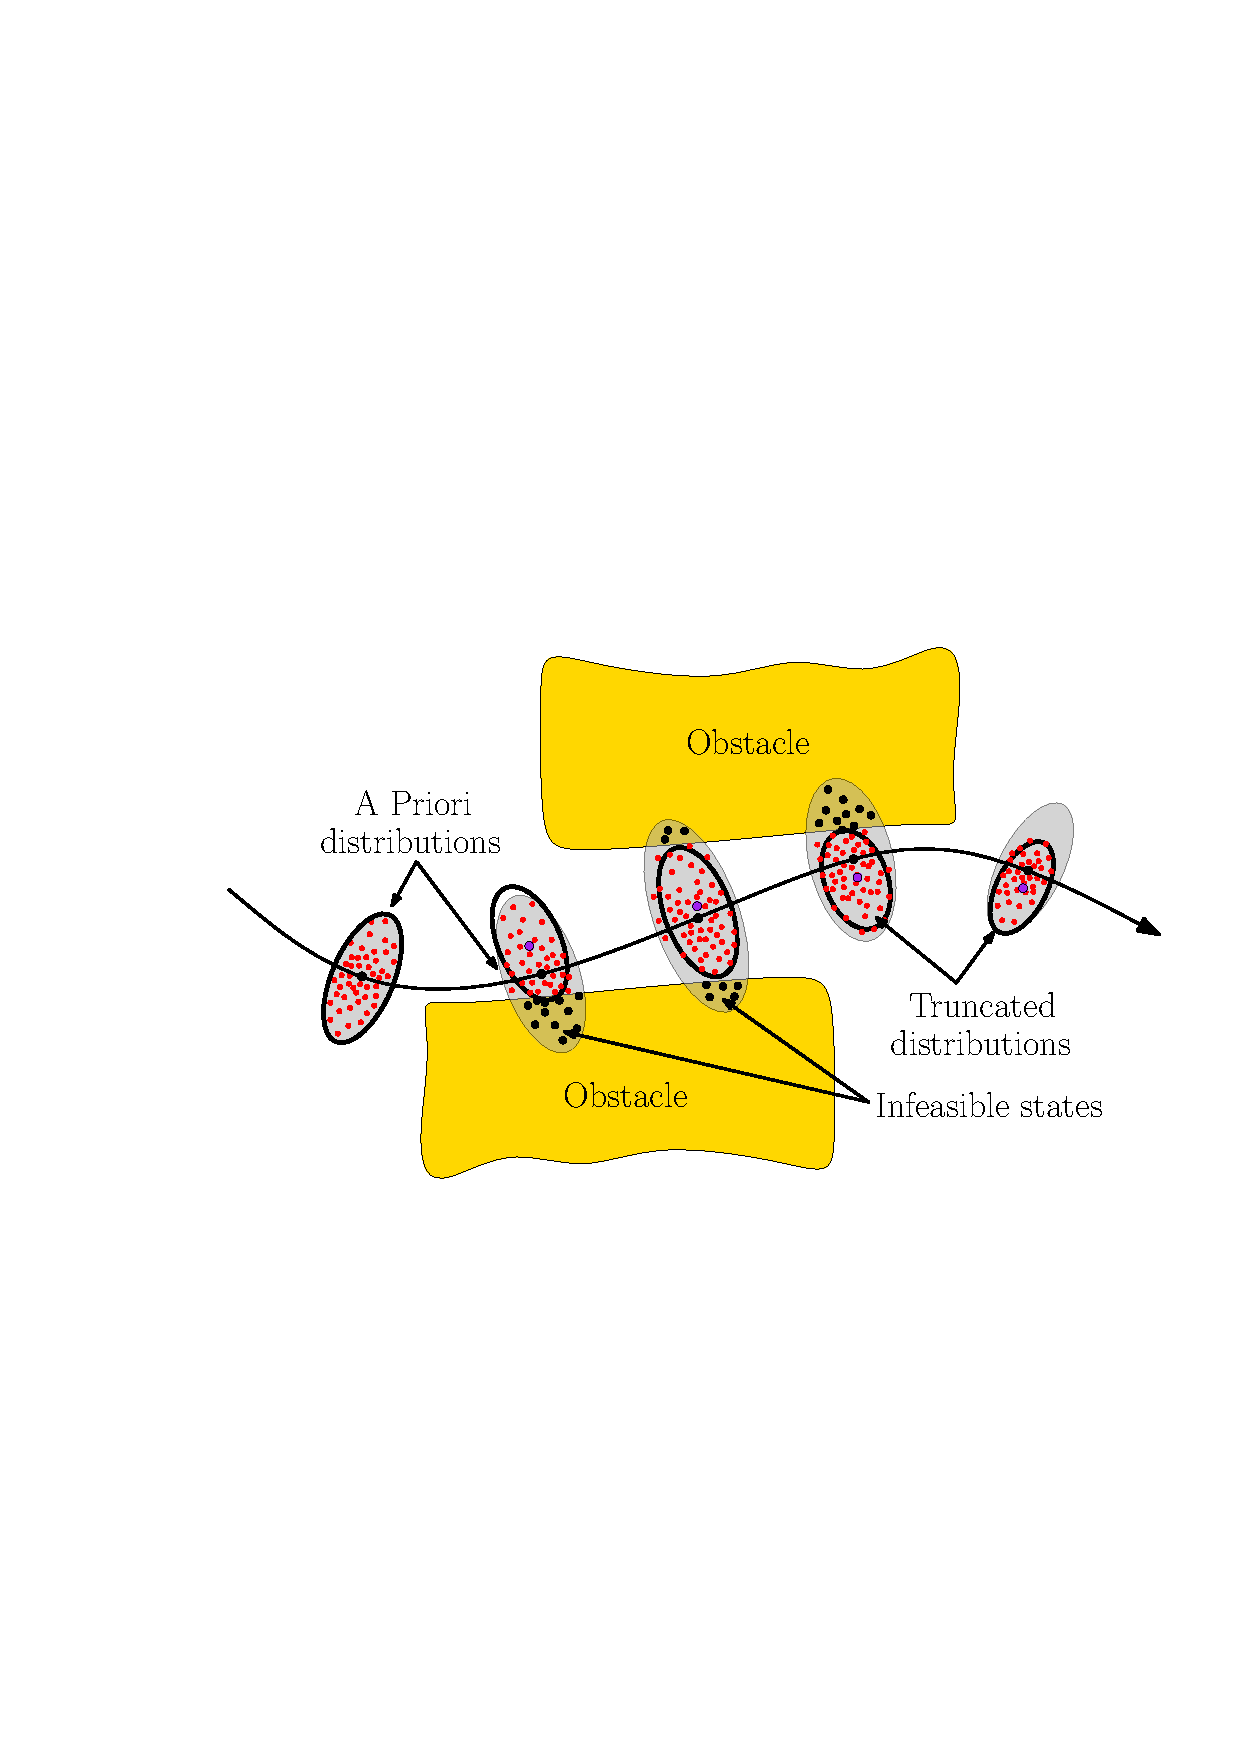
\includegraphics[width=225pt,clip]{figures/truncatedGaussians3.pdf}
\vspace{-5pt}
\caption{We estimate the probability of collision for a motion plan based on \emph{a priori} probability distributions of the robot state. The probability of collision at each stage of the plan is conditioned on the previous stages being collision free. We compute truncated \emph{a priori} distributions that discount plan executions (black dots) that collide with obstacles. Propagating the truncated distributions (black ellipses) accounts for only the collision free samples (red dots), resulting in accurate estimation of the probability of collision. Prior methods that use the unconditional distributions (gray ellipses) to estimate the collision probability result in an overly conservative estimate.}
\label{fig:teaser}
\vspace*{-15pt}
\end{figure}

Prior work on motion planning under uncertainty has used both sampling-based and analytical approaches to estimating probability of collision. Na\"{i}ve Monte Carlo sampling strategies can estimate the probability of collision by computing the ratio of the number of simulated executions that are collision free. This approach requires a large number of simulations to obtain a reliable estimate, which requires more computation time than analytical approaches. Monte Carlo sampling also offers no guarantee that it will not underestimate the probability of collision, resulting in violation of safety requirements.
Under the assumption of Gaussian motion and sensing uncertainty, probability of collision can be estimated quickly based on \emph{a priori} probability distributions of the robot state \cite{vandenBerg11_IJRR, Bry11_ICRA, Vitus11_ICRA}. However, prior methods typically ``approximate'' the collision probability of a plan by assuming the probabilities of collision at stages along the plan are independent. Formally speaking, let $\mathbf{x}_t \in \mathcal{X}$ denote the state of the robot at stage $t$ along the plan, and $\mathcal{X}_{F} \subset \mathcal{X}$ denote the feasible space not occupied by obstacles. Prior methods assume that the probability that a plan consisting of $\ell$ stages is collision free is given by $p(\bigwedge_{t = 0}^{\ell} \; \mathbf{x}_t \in \mathcal{X}_{F}) \approx \prod_{t = 0}^\ell p(\mathbf{x}_{t} \in \mathcal{X}_{F})$. This yields an overly conservative estimate of the probability of collision (see Fig.\ \ref{fig:teaser}), which might result in overly conservative motion plans and, depending on the safety required by the motion planner, may result in failure to find a feasible plan even if one exists.

We propose an analytic approach to estimating the probability of collision that accounts for the fact that the distribution of the state at each stage along the plan is \emph{conditioned} on the previous stages being collision free, i.e., the probability that a plan is collision free is given by $p(\bigwedge_{t = 0}^{\ell}\; \mathbf{x}_t \in \mathcal{X}_{F}) = \prod_{t = 0}^\ell p(\mathbf{x}_{t} \in \mathcal{X}_{F}\; |\; \bigwedge_{i = 0}^{t-1} \; \mathbf{x}_i \in \mathcal{X}_{F})$. This amounts to propagating the \emph{a priori} distributions forward in time in such a way that instances that collide with obstacles are discounted from the propagation (Fig.\ \ref{fig:teaser}). For this we propose a novel method to truncate the \emph{a priori} distributions with respect to obstacles, approximate the truncated distributions by Gaussians, and propagate the truncated distributions forward in time. This results in an accurate estimate of the conditional distributions, and consequently, enables accurate estimation of the collision probability.

%Even though the exposition outlines a method to truncate the distributions with respect to obstacles, we can directly apply this methodology to estimate the \emph{a priori} distributions with other constraints on the state variables (such as imposing limits on velocity, acceleration etc. of the robot).
Our method can be used to quantify the safety of a plan \cite{vandenBerg11_IJRR, Patil11_RSS}, to improve quality of estimation of collision chance constraints \cite{Bry11_ICRA, Vitus11_ICRA}, or to elegantly account for hard state constraints imposed by obstacles in optimization based \cite{Erez10_UAI} or inference based \cite{Toussaint09_ICML} planning methods. Our truncation approach is also directly applicable to the important problem of optimal state estimation with hard state constraints \cite{Book:Simon06}.

We present simulation-based results for two scenarios with with stochastic dynamics and partial, noisy state feedback: (1) a car-like robot with second-order dynamics, and (2) a nonholonomic bevel-tip flexible needle. Our method was orders of magnitude faster than na\"{i}ve sampling based methods and computed a significantly more accurate estimate of collision probability compared to prior analytical methods.


\section{Previous Work} \label{sec:prevwork}
% !TEX root =  ICRA2012-Patil.tex

%Explicitly considering uncertainty in robot motion and sensing during motion planning enables the computation of safer plans.

Motion planners that consider uncertainty have been developed for a variety of applications \cite{Alterovitz07_RSS, Kurniawati08_RSS, Guibas08_WAFR, Prentice09_IJRR, Platt10_RSS, vandenBerg11_IJRR, Patil11_RSS, Bry11_ICRA, Vitus11_ICRA}.
%
A key step of many motion planning methods that consider uncertainty is to estimate the probability of collision of a motion plan. Monte Carlo sampling strategies have been used to accurately estimate this probability \cite{Lambert06_ICARV, duToit11_TRO}. Other methods characterize the uncertainty by estimating the \emph{a priori} probability distributions of the robot state along a given plan. One approach is to check for collisions between these distributions and obstacles is to compute an upper bound for the collision probability for use as a metric to evaluate plan safety \cite{vandenBerg11_IJRR, Patil11_RSS}. Another approach is to use these distributions to compute a conservative probability bound using Boole's inequality \cite{Vitus11_ICRA, Bry11_ICRA}. However, these methods incorrectly assume that the probabilities of collision are independent, which results in overly conservative plans.%, or in some cases, might result in failure to find a feasible plan even if one exists.

The use of truncated Gaussian distributions \cite{Book:Johnson94} has been previously explored in the context of optimal state estimation with state constraints \cite{Book:Simon06}, but this work does not consider motion uncertainty. Greytak \cite{Thesis:Greytak09} provides an analytical method to compute the probability of collision using truncated Gaussians but does not consider sensing uncertainty. %and only truncates the state distributions with respect to the obstacle closest to the robot state being considered.
Toussaint \cite{Toussaint09_ICML} uses truncated Gaussians in an expectation-propagation framework for Bayesian inference, but the truncation result is dependent on the order in which constraints are processed, which leads to problems with convergence of the algorithm \cite{Toussaint09_NIPS}. In contrast, we propose a novel order-independent algorithm for truncating Gaussian distributions with respect to hard state constraints. 

%\section{Problem Statement} \label{sec:problem}
%% !TEX root =  ICRA2012-Patil.tex

We consider a robot operating in an environment that may contain obstacles. The stochastic dynamics of the robot follow a given discrete-time model:
\begin{equation} \label{eq:dynmodel}
\mathbf{x}_{t} = \mathbf{f}[\mathbf{x}_{t-1}, \mathbf{u}_{t-1}, \mathbf{m}_t], ~ \mathbf{m}_t \sim \mathcal{N} [\mathbf{0}, M_t]
\end{equation}
where $\mathbf{x}_t \in \mathcal{X} \subset \mathbb{R}^{n_x}$ is the state of the robot at stage $t$, $\mathbf{u}_t \in \mathbb{R}^{n_u}$ is the applied control input, and $\mathbf{m}_t$ is zero-mean Gaussian noise with variance $M_t$ that models the motion uncertainty. During execution of a plan, partial and noisy sensor measurements of the robot state are available according to a given stochastic model:
\begin{equation}\label{eq:obsmodel}
\mathbf{z}_t = \mathbf{h}[\mathbf{x}_t, \mathbf{n}_t], ~ \mathbf{n}_t \sim \mathcal{N}[\mathbf{0}, N_t]
\end{equation}
where $\mathbf{z}_t \in \mathbb{R}^{n_z}$ is the measurement obtained at time $t$ and $\mathbf{n}_t$ is the zero-mean Gaussian noise with variance $N_t$ that models the sensing uncertainty.

Since our method serves as an evaluation metric, we assume the existence of a nominal plan computed by an RRT or other method as discussed in Sec.\ \ref{sec:prevwork}. The nominal plan is defined by $[\mathbf{x}^{\star}_{0}, \mathbf{u}^{\star}_{0}, \hdots, \mathbf{x}^{\star}_{\ell}, \mathbf{u}^{\star}_{\ell}]$ where $\mathbf{x}^{\star}_{t} = \mathbf{f}[\mathbf{x}^{\star}_{t-1}, \mathbf{u}^{\star}_{t-1}, \mathbf{0}]$ for $0 < t \leq \ell$, where $\ell$ is the number of discrete stages in the plan. The nominal plan is consistent with the dynamics model if there were no motion uncertainty. During actual execution of the plan, the robot will likely deviate from the nominal plan due to motion uncertainty and inaccurate estimation of the robot state due to sensing uncertainty.

To compensate for uncertainty, we assume the robot executes the plan in a closed-loop fashion using a feedback controller and state estimator framework \cite{Book:Stengel94}. We assume the existence of a linear feedback control law that operates on the estimate of the robot state and aims to keep the robot close to the nominal plan. Several feedback controllers, such as the linear quadratic regulator (LQR) and the proportional integral derivative (PID) controller fall in this category and are compatible with our method \cite{Book:Stengel94}. We also assume that a Kalman filter is used for state estimation during execution, which is the minimum mean square error estimator for linear, Gaussian systems. Several variants of the Kalman filter such as the extended filter (EKF), unscented filter (UKF), and the ensemble filter (EnKF) \cite{Book:Simon06} are compatible with our method.

Given Gaussian models of motion and sensing uncertainty, a description of the obstacles in the environment, a nominal motion plan, and associated feedback controller and state estimator, the objective is to compute the probability of collision of a given plan. It is important to note that our method can be directly used for estimating the a priori distributions of the robot's state over time with hard state constraints, which is a key step in several optimization based methods for motion planning under uncertainty. 

\section{Estimating Probability of Collision} \label{sec:probcol}
% !TEX root =  ICRA2012-Patil.tex

\subsection{Problem Statement}

We consider a robot operating in an environment that may contain obstacles.
The stochastic dynamics of the robot follow the given discrete-time model:
\begin{equation} \label{eq:dynmodel}
\mathbf{x}_{t} = \mathbf{f}[\mathbf{x}_{t-1}, \mathbf{u}_{t-1}, \mathbf{m}_t], ~ \mathbf{m}_t \sim \mathcal{N} [\mathbf{0}, M_t]
\end{equation}
where $\mathbf{x}_t \in \mathcal{X} \subset \mathbb{R}^{n_x}$ is the state of the robot at stage $t$, $\mathbf{u}_t \in \mathbb{R}^{n_u}$ is the applied control input, and $\mathbf{m}_t$ is zero-mean Gaussian noise with variance $M_t$ that models the motion uncertainty. During execution of a plan, partial and noisy sensor measurements of the robot state are obtained:
\begin{equation}\label{eq:obsmodel}
\mathbf{z}_t = \mathbf{h}[\mathbf{x}_t, \mathbf{n}_t], ~ \mathbf{n}_t \sim \mathcal{N}[\mathbf{0}, N_t]
\end{equation}
where $\mathbf{z}_t \in \mathbb{R}^{n_z}$ is the measurement obtained at time $t$ and $\mathbf{n}_t$ is the zero-mean Gaussian noise with variance $N_t$ that models the sensing uncertainty.

Since our method serves as an evaluation metric, we assume the existence of a nominal plan computed by a motion planner.
The nominal plan is defined by $[\mathbf{x}^{\star}_{0}, \mathbf{u}^{\star}_{0}, \hdots, \mathbf{x}^{\star}_{\ell}, \mathbf{u}^{\star}_{\ell}]$ where $\mathbf{x}^{\star}_{t} = \mathbf{f}[\mathbf{x}^{\star}_{t-1}, \mathbf{u}^{\star}_{t-1}, \mathbf{0}]$ for $0 < t \leq \ell$, where $\ell$ is the number of discrete stages in the plan.

During actual execution of the plan, the robot will likely deviate from the nominal plan due to motion uncertainty and inaccurate estimation of the robot state due to sensing uncertainty. To compensate for uncertainty, we assume the robot executes the plan in a closed-loop fashion using a feedback controller and state estimator framework \cite{Book:Stengel94}. We assume the existence of a linear feedback control law that operates on the estimate of the robot state and aims to keep the robot close to the nominal plan. %Several feedback controllers, such as the linear quadratic regulator (LQR) and the proportional integral derivative (PID) controller fall in this category and are compatible with our method \cite{Book:Stengel94}.
We also assume that a Kalman filter is used for state estimation during execution. %, which is the minimum mean square error estimator for linear, Gaussian systems. Several variants of the Kalman filter such as the extended filter (EKF), unscented filter (UKF), and the ensemble filter (EnKF) \cite{Book:Simon06} are compatible with our method.
The objective of our method is to then estimate the probability of collision of a given plan.

%\noindent{\textbf{Objective:}} Given Gaussian models of motion and sensing uncertainty, a description of the obstacles in the environment, a nominal motion plan, and associated feedback controller and state estimator, the objective is to compute the probability of collision of a given plan. %It is important to note that our method can be directly used for estimating the \emph{a priori} distributions of the robot's state over time with hard state constraints, which is a key step in several optimization based methods for motion planning under uncertainty.

\begin{figure*}[t]
\centering
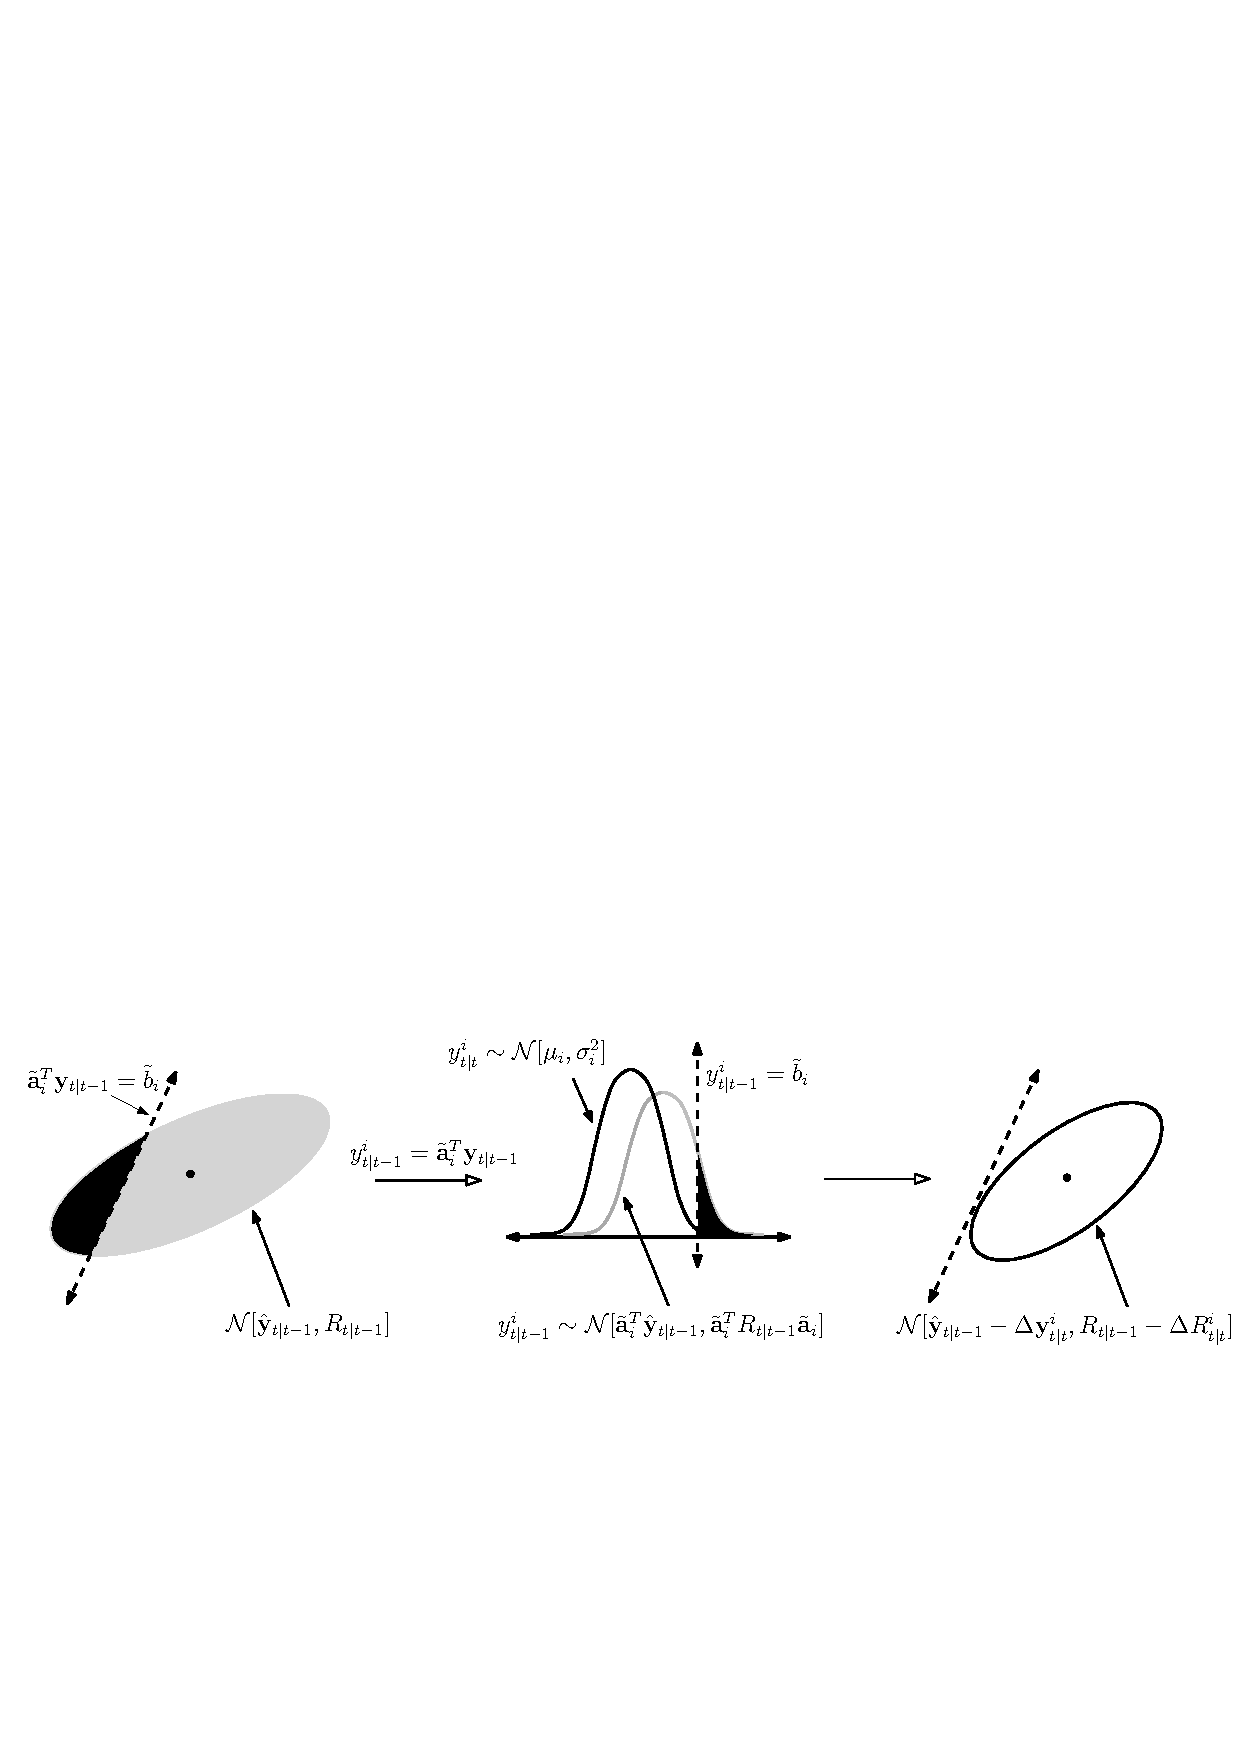
\includegraphics[width=440pt,clip]{figures/truncation2.pdf}
\vspace{-5pt}
\caption{The joint conditional distribution $\mathbf{y}_{t|t-1} \sim \mathcal{N}[\hat{\mathbf{y}}_{t|t-1}, R_{t|t-1}]$ (left), is truncated with respect to the $i^\textrm{th}$ constraint $\tilde{\mathbf{a}}_i^T \mathbf{y}_{t|t-1} \leq \tilde{b}_i$, in $\mathbb{R}^{2n_x}$. Applying an affine transformation, $y^i_{t|t-1} = \tilde{\mathbf{a}}_i^T\mathbf{y}_{t|t-1}$, transforms the distribution to a 1D Gaussian $y_{t|t-1}^i \sim \mathcal{N}[\tilde{\mathbf{a}}_i^T\hat{\mathbf{y}}_{t|t-1}, \tilde{\mathbf{a}}_i^T R_{t|t-1} \tilde{\mathbf{a}}_i]$ (middle). The area under the 1D Gaussian that lies beyond the constraint $y^i_{t|t-1} = \tilde{b}_i$ (shaded in black), gives the probability of collision of the robot with the $i^\textrm{th}$ constraint. We estimate the truncated distribution in $\mathbb{R}^{2n_x}$ by conditioning on the truncated 1D Gaussian $y_{t|t}^i \sim \mathcal{N}[\mu_i, \sigma_i^2]$ (right). The mean $(\hat{\mathbf{y}}_{t|t-1} - \Delta \mathbf{y}_{t|t}^i)$, and variance $(R_{t|t-1} - \Delta R_{t|t}^i)$, of the distribution $\mathbf{y}_{t|t}$ after truncation are obtained by accumulating the effects of truncation with respect to all constraints (order independent).}
\label{fig:truncation}
\vspace*{-10pt}
\end{figure*}

\subsection{A Priori State Distributions}

Since the robot will be controlled to stay close to the nominal plan during execution, we linearize the nonlinear dynamics and measurement models around the plan and express them in terms of deviation from the true state $\bar{\mathbf{x}}_t = (\mathbf{x}_t - \mathbf{x}^{\star}_{t})$, control input deviation $\bar{\mathbf{u}}_t = (\mathbf{u}_t - \mathbf{u}^{\star}_{t})$, and deviation from the actual measurement $\bar{\mathbf{z}}_t = (\mathbf{z}_t - \mathbf{h}[\mathbf{x}^{\star}_{t}, \mathbf{0}])$, as:
\begin{align}
\bar{\mathbf{x}}_t &= A_t\bar{\mathbf{x}}_{t-1} + B_t\bar{\mathbf{u}}_{t-1} + V_t\mathbf{m}_t, ~~ \mathbf{m}_t \sim \mathcal{N} [\mathbf{0}, M_t] \label{eq:lindynmodel} \\
\bar{\mathbf{z}}_t &= H_t\bar{\mathbf{x}}_{t} + W_t\mathbf{n}_t, ~~~~~~~~~~~~~~~~ \mathbf{n}_t \sim \mathcal{N} [\mathbf{0}, N_t]. \label{eq:linobsmodel}
\end{align}
where the Jacobians matrices of $\mathbf{f}$ and $\mathbf{h}$ are given by:
\begin{align} \label{eq:jacobians}
& ~~~~~ A_t = \frac{\partial\mathbf{f}}{\partial\mathbf{x}}[\mathbf{x}^{\star}_{t-1}, \mathbf{u}^{\star}_{t-1},\mathbf{0}], ~ B_t = \frac{\partial\mathbf{f}}{\partial\mathbf{u}}[\mathbf{x}^{\star}_{t-1}, \mathbf{u}^{\star}_{t-1},\mathbf{0}],\\
& V_t = \frac{\partial\mathbf{f}}{\partial\mathbf{m}}[\mathbf{x}^{\star}_{t-1}, \mathbf{u}^{\star}_{t-1},\mathbf{0}],~ H_t = \frac{\partial\mathbf{h}}{\partial\mathbf{x}}[\mathbf{x}^{\star}_{t}, \mathbf{0}],~ W_t = \frac{\partial\mathbf{h}}{\partial\mathbf{n}}[\mathbf{x}^{\star}_{t}, \mathbf{0}] \nonumber.
\end{align}

The true state $\mathbf{x}_t$, and hence the true state deviation $\bar{\mathbf{x}}_t$, is not available during actual execution. We use a Kalman filter to keep track of an estimate of the state deviation $\hat{\mathbf{x}}_t = \mathrm{E}[\bar{\mathbf{x}}_t]$. The estimate of the state deviation evolves according to:
\vspace*{-3pt}
\begin{equation} \label{eq:Kalman}
\hat{\mathbf{x}}_t = K_t\bar{\mathbf{z}}_t + (I - K_tH_t)(A_t \hat{\mathbf{x}}_{t-1} + B_t \bar{\mathbf{u}}_{t-1}),
\end{equation}
where $K_t$ is the Kalman gain matrix \cite{Book:Simon06}. To compensate for the uncertainty, we assume that the robot is controlled using a linear feedback policy related to the estimate of the state deviation as:
\vspace*{-3pt}
\begin{equation} \label{eq:controlpolicy}
\bar{\mathbf{u}}_t = L_{t+1}\hat{\mathbf{x}}_{t},
\end{equation}
where $L_t$ is the control gain matrix determined by the choice of feedback controller \cite{Book:Stengel94}.

Under the given assumptions, the probability distributions of the robot state can be characterized \emph{a priori}, i.e. before execution. Combining Eqns. (\ref{eq:lindynmodel}), (\ref{eq:linobsmodel}), (\ref{eq:Kalman}), and (\ref{eq:controlpolicy}), the true state deviation $\bar{\mathbf{x}}_t$, and the estimate $\hat{\mathbf{x}}_t$, jointly evolve as \cite{vandenBerg11_IJRR}:
\begin{align}\label{eq:jointevolve}
\begin{bmatrix} \bar{\mathbf{x}}_t \\ \hat{\mathbf{x}}_t \end{bmatrix} =& \begin{bmatrix} A_t & B_tL_t \\ K_tH_tA_t & A_t + B_tL_t - K_tH_tA_t \end{bmatrix} \begin{bmatrix} \bar{\mathbf{x}}_{t-1} \\ \hat{\mathbf{x}}_{t-1} \end{bmatrix} + \\ & \begin{bmatrix} V_t & 0 \\ K_tH_tV_t & K_tW_t \end{bmatrix} \begin{bmatrix} \mathbf{m}_t \\ \mathbf{n}_t \end{bmatrix}, ~ \begin{bmatrix} \mathbf{m}_t \\ \mathbf{n}_t \end{bmatrix} \sim \mathcal{N}[\mathbf{0}, \begin{bmatrix} M_t & 0 \\ 0 & N_t \end{bmatrix}] \nonumber.
\end{align}
We can write this equation in shorthand (for appropriate definitions of $\mathbf{y}_t$, $\mathbf{q}_t$, $F_t$, $G_t$, and $Q_t$) as:
\begin{equation}
\mathbf{y}_t = F_t\mathbf{y}_{t-1} + G_t\mathbf{q}_{t}, ~ \mathbf{q}_t \sim \mathcal{N}[\mathbf{0}, Q_t].
\end{equation}
The mean $\hat{\mathbf{y}}_t \in \mathbb{R}^{2n_x}$ and associated variance $R_t = \mathrm{Var}[\mathbf{y}_t]$, propagate according to:
\begin{align}
\hat{\mathbf{y}}_t &= F_t\hat{\mathbf{y}}_{t-1}, ~~~~~~~~~~~~~~~~~~~ \hat{\mathbf{y}}_0 = \mathbf{0}, \label{eq:oldjointmean}\\
R_t &= F_tR_{t-1}F_t^T + G_tQ_tG_t^T, ~~ R_0 = \begin{bmatrix} \mathrm{Var}[\bar{\mathbf{x}}_0] & 0 \\ 0 & 0 \end{bmatrix}. \label{eq:oldjointvar}
\end{align}
The \emph{unconditional} \emph{a priori} distribution of the state $\mathbf{x}_t$ at stage $t$ is then given by the marginal $\mathbf{x}_t \sim \mathcal{N}[(\mathbf{x}^{\star}_t + \Lambda \hat{\mathbf{y}}_t), \Lambda R_t \Lambda^T]$, where $\Lambda = \left[ I ~~ 0  \right]$. %The unconditional distribution assumes that the probabilities of collision are independent at each stage of the plan.

To accurately estimate the probability of collision, we need to estimate the \emph{a priori} state distributions at each stage along the plan that are \emph{conditioned} on the previous stages being collision free, i.e. the distributions $(\mathbf{x}_t\;|\;\bigwedge_{i=0}^{t-1}\; \mathbf{x}_i \in \mathcal{X}_F)$. To this end, we pursue a recursive approach similar as above to propagate the conditional distributions.

Let $\mathbf{y}_{t|s}$ denote the joint distribution of the true state deviation and its estimate at time $t$ conditioned on the state being collision free for all stages $0,\ldots,s$:
\begin{align}
\mathbf{y}_{t|s} = (\begin{bmatrix} \bar{\mathbf{x}}_t \\ \hat{\mathbf{x}}_t \end{bmatrix} \; | \; \bigwedge_{i=0}^s \; \mathbf{x}_i \in \mathcal{X}_F).
\end{align}
We then repeatedly, for each stage $t$ of the plan, carry out the following steps. Assume we are given the joint conditional distribution $\mathbf{y}_{t|t-1}$ as approximated by a Gaussian distribution $\mathcal{N}[\hat{\mathbf{y}}_{t|t-1}, R_{t|t-1}]$. We then approximate the distribution $\mathbf{y}_{t|t}  \sim \mathcal{N}[\hat{\mathbf{y}}_{t|t}, R_{t|t}]$ of all collision-free states at stage $t$ by truncating the distribution $\mathbf{y}_{t|t-1}$ against the obstacles in the environment. Truncating the distribution effectively discounts all colliding states from the distribution (Fig.\ \ref{fig:teaser}), and results in a shift of the mean and variance by $\Delta \mathbf{y}_t$ and $\Delta R_t$ (as detailed in Sec.\ \ref{sec:trunc}), respectively:
\begin{align}
\hat{\mathbf{y}}_{t|t} & = \hat{\mathbf{y}}_{t|t-1} - \Delta \mathbf{y}_t \\
R_{t|t} & = R_{t|t-1} - \Delta R_t
\end{align}
Using Eqns. (\ref{eq:oldjointmean}) and (\ref{eq:oldjointvar}), the conditional mean and variance are then propagated according to:
\begin{align}
\hat{\mathbf{y}}_{t+1|t} &= F_{t+1} \hat{\mathbf{y}}_{t|t}, \label{eq:newjointmean}\\
R_{t+1|t} &= F_{t+1}R_{t|t}F_{t+1}^T + G_{t+1}Q_{t+1}G_{t+1}^T. \label{eq:newjointvar}
\end{align}
The recursion then continues. The initial conditions are set by defining $\hat{\mathbf{y}}_{0|-1} = \hat{\mathbf{y}}_0 = \mathbf{0}$ and $R_{0|-1} = R_0 = \left[\begin{smallmatrix} \mathrm{Var}[\bar{\mathbf{x}}_0] & 0 \\ 0 & 0 \end{smallmatrix} \right]$.

At each stage of the recursion, the marginal $\mathbf{x}_{t|t-1} \sim \mathcal{N}[(\mathbf{x}^{\star}_t + \Lambda \hat{\mathbf{y}}_{t|t-1}), \Lambda R_{t|t-1} \Lambda^T]$ of the joint distribution $\mathbf{y}_{t|t-1}$ gives the \emph{a priori} distribution of the robot state $\mathbf{x}_t$ given that all the previous states $[\mathbf{x}_0,\ldots,\mathbf{x}_{t-1}]$ are collision free. %When this distribution is truncated against the obstacles, an accurate estimate is obtained of the conditional probability of collision at stage $t$ (as detailed in Sec.\ \ref{sec:estprob}).

\subsection{Truncating A Priori Distributions} \label{sec:trunc}

At each stage $t$ of the plan, we approximate the distribution of the feasible robot states with a truncated Gaussian distribution \cite{Book:Johnson94}. For the sake of brevity, we assume that the feasible region containing the state at each stage $t$ is convex and is described by the conjunction of $k$ linear inequality constraints as $\bigcap_{i = 0}^{k}\; \mathbf{a}_i\mathbf{x}_t \leq b_i$. We later extend this analysis in Sec. \ref{sec:cvxfn} to non-convex regions by constructing a locally convex feasible region around the robot state.

Since the true state deviation and its estimate are correlated (Eqn.\ \ref{eq:jointevolve}), it is important to truncate the joint conditional distribution $\mathcal{N}[\hat{\mathbf{y}}_{t|t-1}, R_{t|t-1}]$ in $\mathbb{R}^{2n_x}$, with respect to the $k$ constraints. The $i^{\textrm{th}}$ linear constraint is then represented in $\mathbb{R}^{2n_x}$ as $\tilde{\mathbf{a}}_i^T \mathbf{y}_{t|t-1} \leq \tilde{b}_i$, where $\tilde{\mathbf{a}}_i = \left[\begin{smallmatrix} \mathbf{a}_i \\ \mathbf{0} \end{smallmatrix} \right]$, and $\tilde{b}_i = (b_i - \mathbf{a}_i^T\mathbf{x}^{\star}_t)$.

We truncate the joint conditional distribution with respect to each constraint in a sequential manner and then accumulate the effect of truncation over all the constraints. In contrast to prior methods that use truncated distributions \cite{Book:Simon06, Toussaint09_NIPS}, we propose a novel truncation method that does not depend on the order in which the constraints are processed. Given the $i^{\textrm{th}}$ constraint $\tilde{\mathbf{a}}_i^T \mathbf{y}_{t|t-1} \leq \tilde{b}_i$, we apply an affine transformation $y^i_{t|t-1} = \tilde{\mathbf{a}}_i^T\mathbf{y}_{t|t-1}$ to transform the conditional distribution $\mathcal{N}[\hat{\mathbf{y}}_{t|t-1}, R_{t|t-1}]$, to a 1D Gaussian $\mathcal{N}[\tilde{\mathbf{a}}_i^T\hat{\mathbf{y}}_{t|t-1}, \tilde{\mathbf{a}}_i^T R_{t|t-1} \tilde{\mathbf{a}}_i]$ along an axis normal to the constraint (as shown in Fig.\ \ref{fig:truncation}). The problem now simplifies to truncating the 1D Gaussian distribution at a specified upper bound given by $y^i_{t|t-1} = \tilde{b}_i$, which is well-known from standard statistical literature \cite{Book:Johnson94}. The mean, $\mu_i$ and variance, $\sigma^2_i$ of the truncated 1D Gaussian $y_{t|t}^i$ is given by:
\begin{align}
\mu_i &= \tilde{\mathbf{a}}_i^T\hat{\mathbf{y}}_{t|t-1} + \lambda(\alpha_i)\sqrt{\tilde{\mathbf{a}}_i^T R_{t|t-1} \tilde{\mathbf{a}}_i}, \label{eq:1DtruncMu}\\
\sigma^2_i &= \tilde{\mathbf{a}}_i^T R_{t|t-1} \tilde{\mathbf{a}}_i (1 - \lambda(\alpha_i)^2 + \alpha_i \lambda(\alpha_i)) \label{eq:1DtruncSigma},
\end{align}
where
\begin{equation} \label{eq:alpha}
\alpha_i = \frac{(\tilde{b}_i - \tilde{\mathbf{a}}_i^T\hat{\mathbf{y}}_{t|t-1})}{\sqrt{\tilde{\mathbf{a}}_i^T R_{t|t-1} \tilde{\mathbf{a}}_i}}, ~~~ \lambda(\alpha_i) = \frac{\textrm{pdf}(\alpha_i)}{\textrm{cdf}(\alpha_i)}.
\end{equation}
Here, $\lambda(\alpha_i)$ is the ratio of the standard Gaussian (mean $0$ and variance $1$) probability distribution function and the standard Gaussian cumulative distribution function evaluated at $\alpha_i$. Note that $(1 - \textrm{cdf}(\alpha_i))$ is the area under the Gaussian that lies beyond the constraint (shaded in black in Fig.\ \ref{fig:truncation}), and is the probability that the robot lies in the infeasible region corresponding to the $i^\textrm{th}$ constraint.
%$\alpha_i = \frac{(\tilde{b}_i - \tilde{\mathbf{a}}_i^T\hat{\mathbf{y}}_t)}{\sqrt{\tilde{\mathbf{a}}_i^T R_t \tilde{\mathbf{a}}_i}}$, and $\lambda(\alpha_i) = \frac{\textrm{pdf}(\alpha_i)}{\textrm{cdf}(\alpha_i)}$, is the ratio of the Gaussian probability distribution function and the Gaussian cumulative distribution function evaluated at $y'_t = \alpha_i$. Note that $(1 - \textrm{cdf}(\alpha_i))$ is the area under the Gaussian (shaded in black in Fig.\ \ref{fig:truncation}) that lies beyond the truncation limit $\tilde{b}_i$, and is the probability that the robot lies in the infeasible region corresponding to the $i^\textrm{th}$ constraint.

The mean and variance of the truncated distribution $\mathbf{y}_{t|t}$ are found by conditioning the joint distribution $(\mathbf{y}_{t|t-1},y^i_{t|t-1})$, on the truncated 1D distribution $y^i_{t|t}$: $\mathbf{y}_{t|t} = (\mathbf{y}_{t|t-1}|y^i_{t|t-1}=y^i_{t|t})$ (see appendix). The shift in the mean due to truncation with respect to the $i^\textrm{th}$ constraint is given by:
\begin{equation} \label{eq:truncmean}
\Delta \mathbf{y}^i_t = \frac{R_{t|t-1}\tilde{\mathbf{a}}_i}{\tilde{\mathbf{a}}_i^T R_{t|t-1} \tilde{\mathbf{a}}_i}(\tilde{\mathbf{a}}_i^T\hat{\mathbf{y}}_{t|t-1} - \mu_i),
\end{equation}
and the shift in variance is given by:
\begin{equation} \label{eq:truncvar}
\Delta R^i_t = \frac{R_{t|t-1}\tilde{\mathbf{a}}_i}{\tilde{\mathbf{a}}_i^T R_{t|t-1} \tilde{\mathbf{a}}_i}(\tilde{\mathbf{a}}_i^TR_{t|t-1}\tilde{\mathbf{a}}_i - \sigma_i^2)\frac{\tilde{\mathbf{a}}_i^TR_{t|t-1}}{\tilde{\mathbf{a}}_i^T R_{t|t-1} \tilde{\mathbf{a}}_i}.
\end{equation}

Given $k$ constraints, the cumulative shift in the mean due to truncation is then given by $\Delta \mathbf{y}_t = \sum_{i = 0}^{k} \Delta \mathbf{y}^i_t$, and the cumulative change in variance is given by $\Delta R_t = \sum_{i = 0}^{k} \Delta R^i_t$. The mean and variance of the truncated conditional distributions are then propagated recursively using Eqs.\ (\ref{eq:newjointmean}) and (\ref{eq:newjointvar}).

%The truncation method described here is general enough to handle constraints on the entire robot state. Examples of such constraints include spatial constraints imposed on the position of the robot by obstacles in the environment or limits imposed on other state variables such as the velocity and acceleration of the robot. Our method had the added advantage that it is independent of the order in which constraints are processed, which eliminates convergence issues related to handling state constraints in several optimization \cite{Erez10_UAI} and inference based \cite{Toussaint09_ICML} planning methods.

\subsection{Estimating the Probability of Collision} \label{sec:estprob}

We use the truncated conditional distributions to estimate the overall probability of collision of the given plan, based on the conditional probabilities of collisions at each stage along the plan. Given the joint conditional distribution at stage $t$, $\mathcal{N}[\hat{\mathbf{y}}_{t|t-1}, R_{t|t-1}]$, and the set of $k$ linear constraints that define the locally convex region of free space containing the robot, we compute a lower bound for the probability of the robot being collision free using Boole's inequality, as \cite{Vitus11_ICRA}:
\begin{align} \label{eq:probboole}
p(\mathbf{x}_{t|t-1} \in \mathcal{X}_{F}) &\geq 1 - p\bigl(\bigvee_{i = 0}^{k} \; \tilde{\mathbf{a}}_i^T \hat{\mathbf{y}}_{t|t-1} > \tilde{b}_i \bigr) \nonumber\\ &
\geq 1 - \sum_{i = 0}^{k} (1 - \textrm{cdf} (\alpha_i)).
\end{align}

The overall probability that the robot does not collide with any obstacle for the duration $\ell$ of the plan, is given by:
\begin{equation} \label{eq:probsuccess}
p(\bigwedge_{t = 0}^{\ell}\; \mathbf{x}_t \in \mathcal{X}_{F}) = \prod_{t = 0}^{\ell} p(\mathbf{x}_{t|t-1} \in \mathcal{X}_{F}),
\end{equation}
and the overall probability of collision is provided by the complement $(1 - p(\bigwedge_{t = 0}^{\ell}\; \mathbf{x}_t \in \mathcal{X}_{F}))$. %Since the probability of the robot being collision-free is a lower bound, the complement provides a conservative upper bound, i.e. it never underestimates the true probability of collision. 

\section{Local Convexification of Free Space} \label{sec:cvxfn}
\begin{figure}[t]
\begin{center}
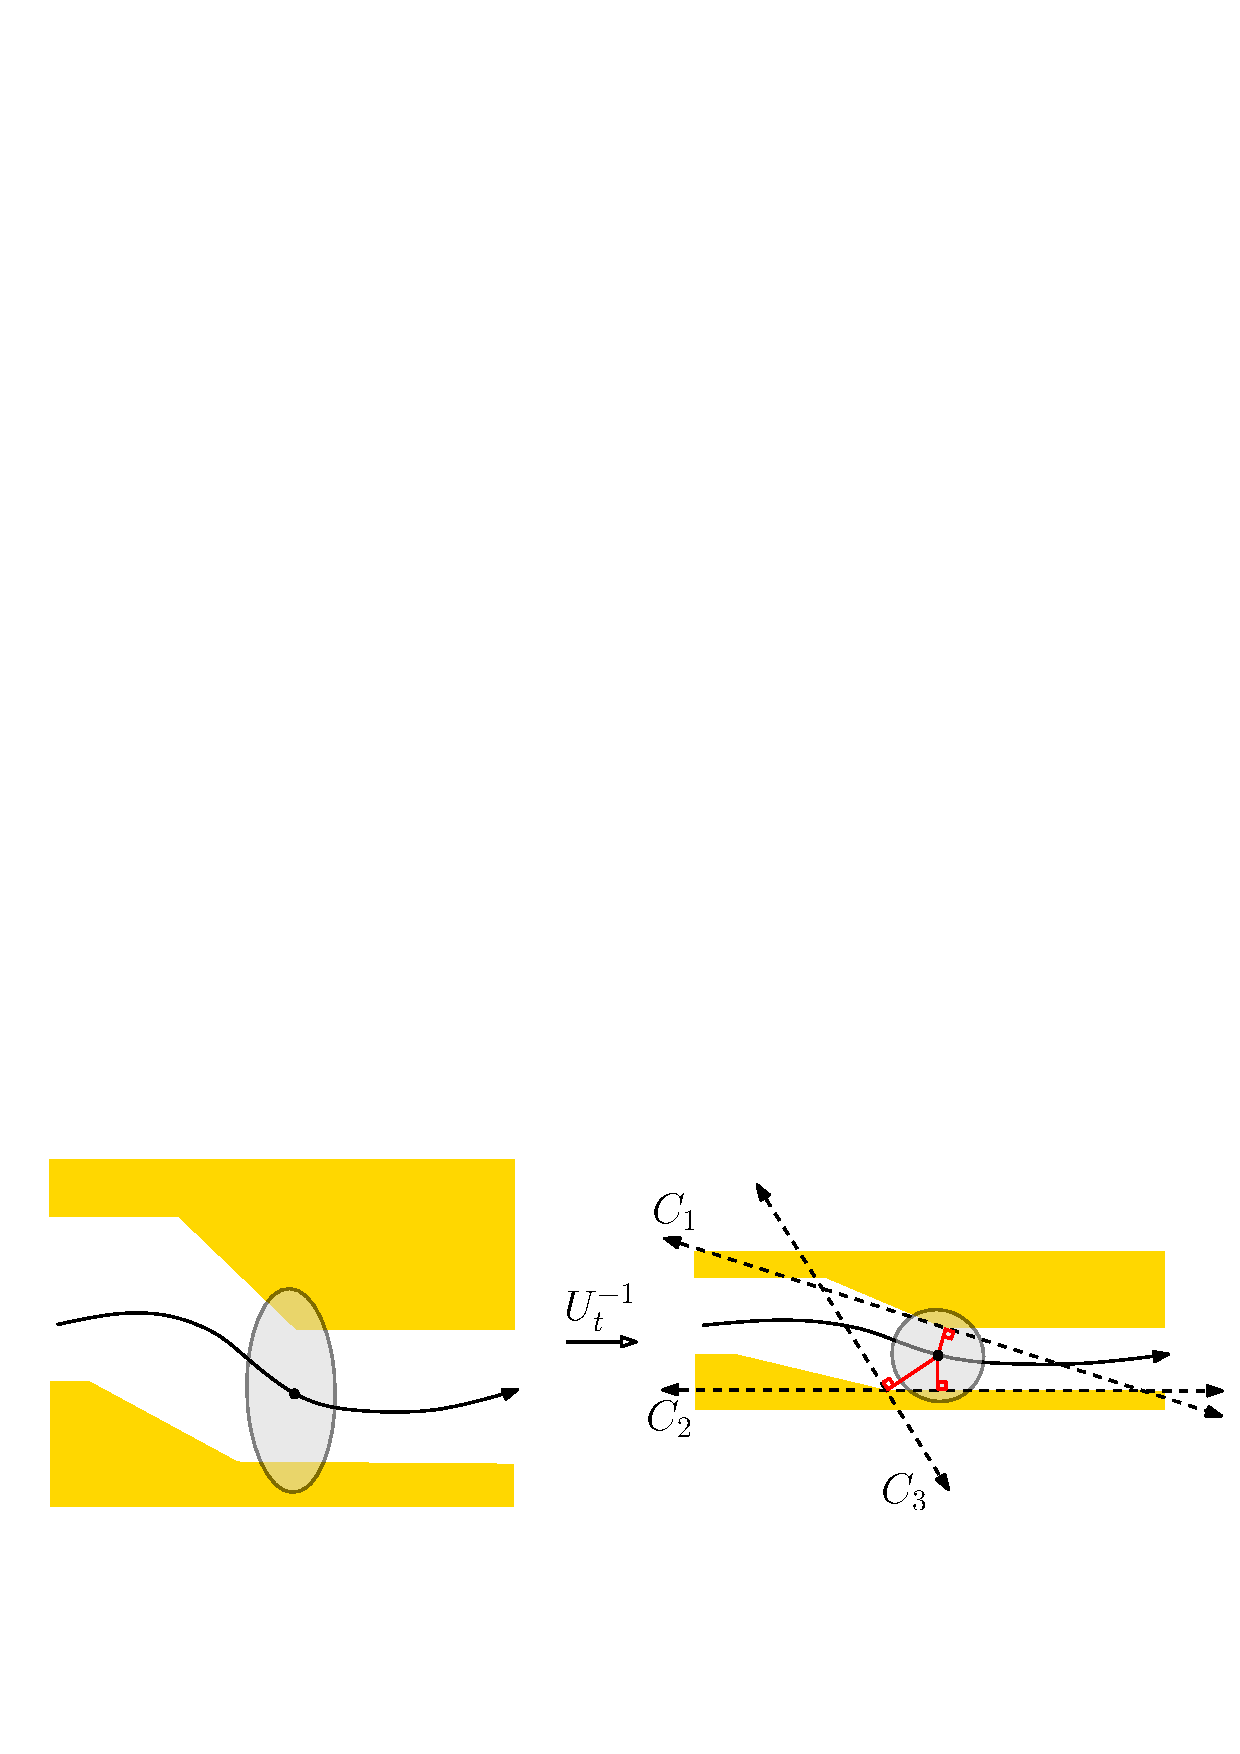
\includegraphics[width=240pt,clip]{figures/convexification.pdf}
\end{center}
\vspace*{-10pt}
\caption{We transform the environment such that the distribution of the robot position (left) is converted to a unit sphere (right). We then sequentially process the obstacle geometry in increasing order of distance from the origin. The linear constraints that define a locally convex region of the free space are determined by the normal to the vector of closest approach (shown in red). The locally convex region constructed using our approach for this example is defined by three constraints determined in order of their indices: $C_1$, $C_2$, and $C_3$.
\vspace*{-10pt}}
\label{fig:convexification}
\end{figure} 

We extend our analysis to non-convex regions by truncating the joint conditional distributions with respect to linear constraints that define a locally convex region of free space containing the robot. For the sake of simplicity, we assume that only the robot position is relevant for collision detection. Given the conditional distribution at stage $t$, $\mathcal{N}[\hat{\mathbf{y}}_{t|t-1} + \bigl[ \begin{smallmatrix} \mathbf{x}^{\star}_t \\ \mathbf{x}^{\star}_t \end{smallmatrix} \bigr], R_{t|t-1}]$, the distribution of the robot position is given by the marginal $\mathcal{N}[\hat{\mathbf{p}}_{t|t-1}, \Sigma_{t|t-1}]$, computed over the state dimensions that describe the robot position. We outline a greedy method that computes a locally convex region of free space such that the probability that the distribution $\mathcal{N}[\hat{\mathbf{p}}_{t|t-1}, \Sigma_{t|t-1}]$ lies beyond the convex region is minimal.

Adopting the approach suggested in \cite{vandenBerg11_IJRR}, we linearly transform the environment geometry by applying the transform $U_t^{-1}$, where $\Sigma_t = U_tU_t^T$ is the Cholesky decomposition. This transforms the uncertainty distribution of the robot position to a Gaussian distribution with zero mean and unit variance, which is a unit sphere in Euclidean space centered at the origin. The spherical symmetry simplifies the task of constructing a nonconservative convex region of free space around the distribution of the position of the robot.

We construct the convex region using a sequential process. We consider the closest point on the obstacle geometry from the origin. The linear truncation constraint $\mathbf{a}_i^T\mathbf{p}_{t|t-1} \leq b_i$, is defined by the normal to the vector of closest approach to the obstacle. We then prune away all geometry that lies in the infeasible half space $\mathbf{a}_i^T \mathbf{p}_{t|t-1} > b_i$ of the constraint, and continue the process by considering the closest point on the remaining obstacle geometry to the origin. This procedure is repeated until all geometry has been pruned away. It is important to note that our convexification method works in a greedy fashion and is not guaranteed to find the least conservative convex bounding region.

In our implementation, we assume that the obstacles are defined in a piecewise linear fashion using either line segments in $\mathbb{R}^2$, or polygons in $\mathbb{R}^3$. We only consider obstacles that are contained within $3$ standard deviations of the distribution (corresponding to a distance of $3$ units from the origin in the transformed environment). Instead of performing a linear-time search by iterating over all obstacles, we use a BSP tree \cite{Book:Berg08} data structure to determine obstacles within the given search radius, in logarithmic time. 

\section{Results} \label{sec:results}
% !TEX root =  ICRA2012-Patil.tex

We present simulation results for two scenarios: a car-like robot with second order dynamics and a nonholonomic bevel-tip flexible needle. In both scenarios, the robot moves subject to stochastic dynamics under the guidance of partial and noisy state measurements. In each case, we initialize our method with a nominal plan computed using an RRT planner \cite{Book:Lavalle06}. We empirically demonstrate that our method provides a more accurate estimation of the a priori probability distributions of the robot state and the probability of collision compared to prior methods. We also validate our method by comparing the estimated collision probability with the probability computed by Monte-Carlo simulations (considered as ground truth). We implemented our method in C++ and tested it on a 3.33 Ghz Intel\textsuperscript{\tiny \textregistered} i7\textsuperscript{\tiny TM} PC.

\subsection{Car-like Robot with Second Order Dynamics}

\begin{figure*}[!t]
{\,} \hfill
\subfigure[\label{fig:1a}]{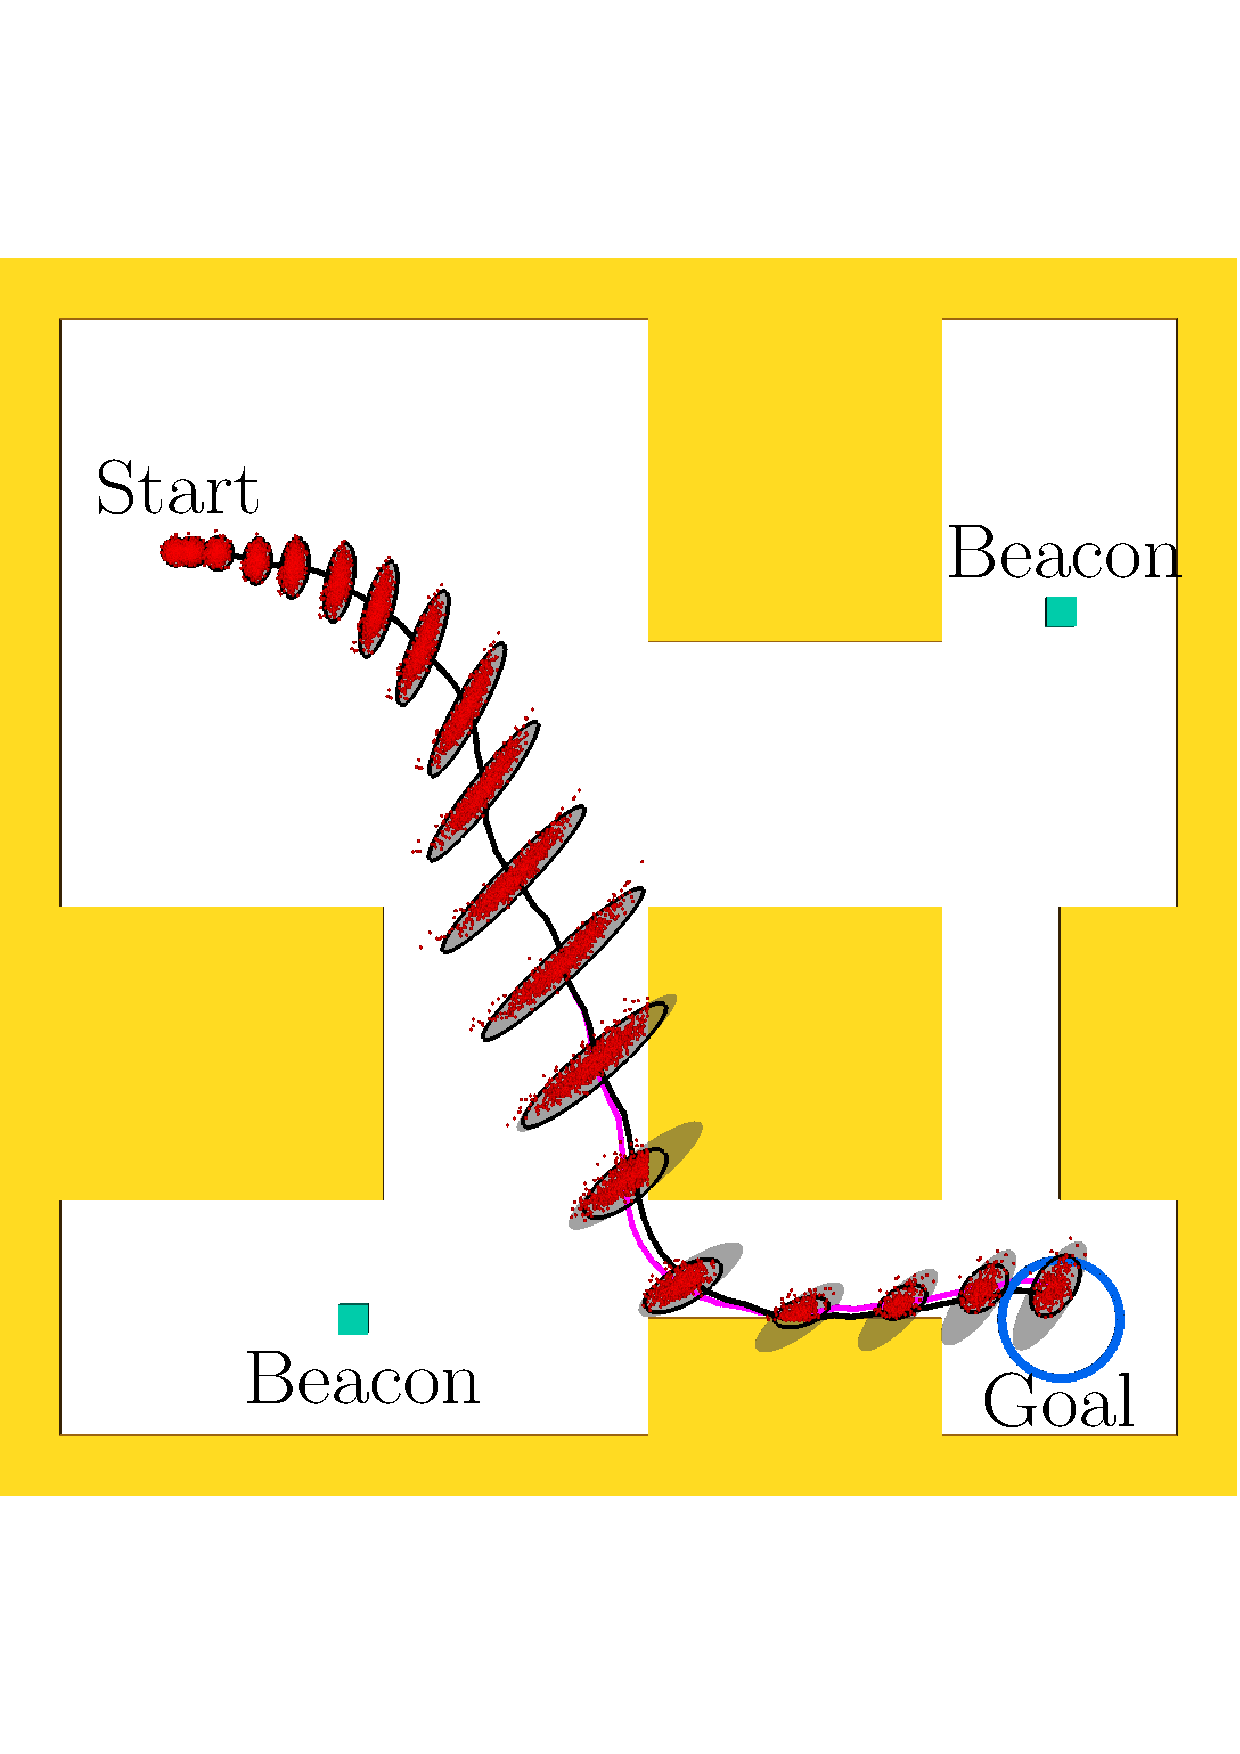
\includegraphics[width=160pt,clip]{figures/car2d/car2d-fig.pdf}}
\hfill
\subfigure[\label{fig:1b}]{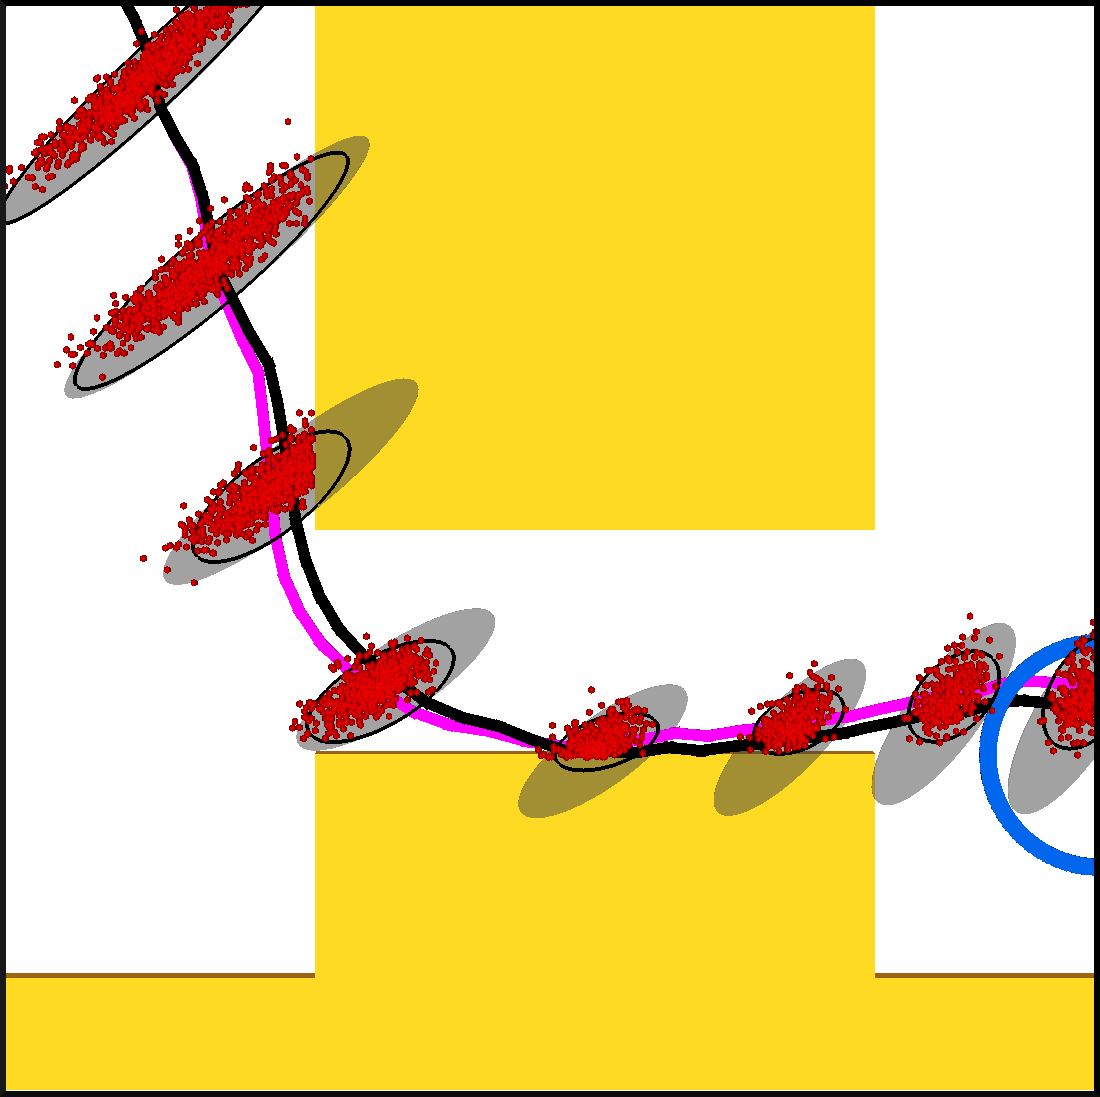
\includegraphics[width=160pt,clip]{figures/car2d/plan1-closeup.png}}
\hfill
\subfigure[\label{fig:1c}]{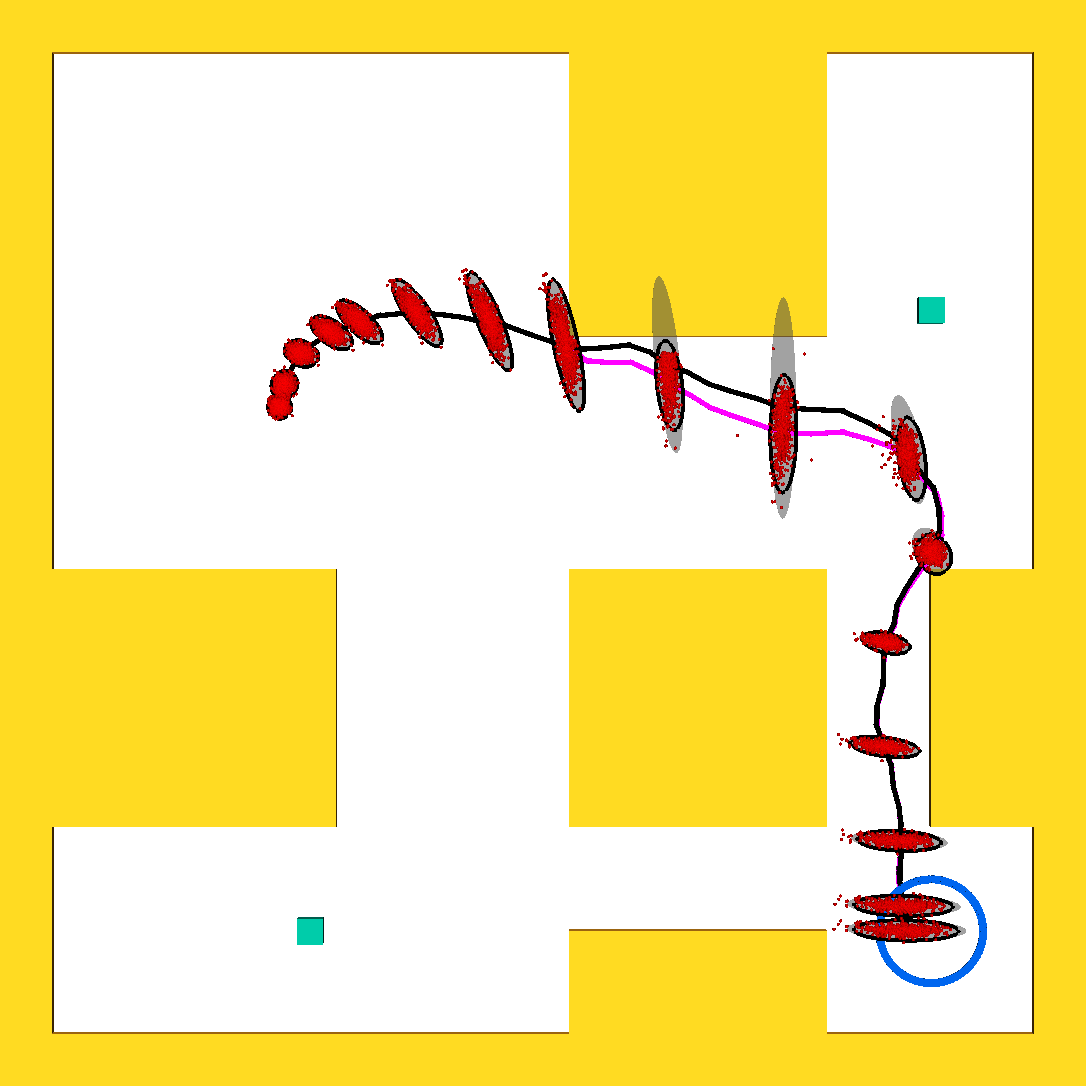
\includegraphics[width=160pt,clip]{figures/car2d/plan3.png}}
{\,} \hfill
\vspace*{-5pt}
\caption{Car-like robot with second order dynamics: (a) An initial plan (black) is computed using an RRT planner. The unconditional distributions (solid gray ellipses showing $3$ standard deviations of the Gaussian distribution) provide an overly conservative approximation of the uncertainty. Samples of the true distribution computed by Monte Carlo simulations are shown by the red dots.
Our method computes conditional distributions (black ellipses showing $3$ standard deviations), which provide an accurate estimate of the true distributions. The probability of collision estimated by our method for this example is $68.87\%$, while the probability determined by Monte-Carlo simulations is $66.26\%$. Our method provides an accurate, yet conservative, approximation of the collision probability. (b) Zoomed in view of the conditional distributions in the narrow corridor in the environment. The mean of the conditional distribution (magenta) deviates from the nominal plan due to the truncation of the distributions due to obstacle collisions. (c) Conditional and unconditional distributions computed along a second plan. The probability of collision estimated by our method for this example is $44.78\%$, while the probability determined by Monte-Carlo simulations is $42.32\%$.}
\vspace*{-15pt}
\label{fig:car2d}
\end{figure*}

We apply our method to a nonholonomic car-like robot with second order dynamics, navigating in a 2D environment with obstacles. The state of the robot, $\mathbf{x} = [x, y, \theta, v]^T \in \mathbb{R}^4$, consists of its position $[x, y]$, its orientation $\theta$, and its speed $v$. The control input $\mathbf{u} = [a, \phi]^T \in \mathbb{R}^2$, consists of the acceleration $a$, and steering angle $\phi$, corrupted by motion noise $\mathbf{m} = [\tilde{a}, \tilde{\phi}]^T \sim \mathcal{N}[\mathbf{0}, M]$. This gives the following stochastic dynamics model:
\begin{equation}
\mathbf{f}[\mathbf{x}, \mathbf{u}, \mathbf{m}] = \begin{bmatrix} x + \tau v \mathrm{cos}\theta \\ y + \tau v \mathrm{sin}\theta \\ \theta + \tau v \mathrm{tan}(\phi + \tilde{\phi})/d \\ v + \tau(a + \tilde{a}) \end{bmatrix},
\end{equation}
where $\tau$ is the time step, and $d$ is the length of the car.

The robot localizes itself using noisy signal measurements from two beacons $b_1$ and $b_2$, placed in the environment at locations $[\check{x}_1, \check{y}_1]$ and $[\check{x}_2, \check{y}_2]$ respectively. The strength of the signal decays quadratically with the distance to the beacon. The robot also measures its current speed using an on-board speedometer. The observation vector $\mathbf{z} \in \mathbb{R}^3$, consists of two readings of signal strengths from the beacons and a speed measurement from the speedometer, corrupted by sensing noise $\mathbf{n} \sim \mathcal{N}[\mathbf{0}, N]$. This gives us the following stochastic measurement model:
\begin{equation}
\mathbf{h}[\mathbf{x}, \mathbf{n}] = \begin{bmatrix} 1/((x - \check{x}_1)^2 + (y - \check{y}_1)^2 + 1) \\ 1/((x - \check{x}_2)^2 + (y - \check{y}_2)^2 + 1) \\ v \end{bmatrix} + \mathbf{n}.
\end{equation}

We consider a non-convex environment with narrow corridors to evaluate the performance of our method (Fig. \ref{fig:1a}). Fig. \ref{fig:1b} shows the discrepancy between the unconditional and conditional distributions in the presence of obstacles. The conditional distributions computed using our method provide an accurate estimate of the distribution of the collision free robot states along the plan, thus providing an accurate estimate of the probability of collision. Fig. \ref{fig:1c} shows how the mean of the conditional distribution can deviate significantly in the close vicinity of obstacles. Interestingly, the conditional and unconditional distributions become identical towards the end of the plan in the absence of obstacles.

To validate our method, we generated a set of $100$ plans using the RRT planner using randomly initialized start states. We estimated the probability of collision using our method for each of these plans. This took $0.09$ seconds. We also used a brute-force approach to estimate the ground truth probability of collision using Monte-Carlo sampling. We performed $10,000$ simulations of executions of each plan using the given controller and Kalman filter, and with artificially generated motion and measurement noise, and counted the number of collision free executions. This took $271$ seconds, which is orders of magnitude slower than our method.

Table~\ref{tab:comp} compares the collision probability estimate computed using our method with the probability computed using brute-force Monte-Carlo sampling, applying Boole's inequality to the unconditional distributions \cite{Vitus11_ICRA}, and LQG-MP \cite{vandenBerg11_IJRR}. We use the mean error as a metric to compare the probability estimates to the ground truth probability computed using sampling, across $100$ randomly generated plans.

For this example, the mean error in estimation using our method as compared to the ground truth probability is $3.0\%$. The estimate computing using our method is much more accurate than the collision quality metric provided by LQG-MP (mean error of $52.2\%$) \cite{vandenBerg11_IJRR} and the collision probability computed using the unconditional distributions directly by assuming independent probabilities (mean error of $28.0\%$) \cite{Vitus11_ICRA}, with negligible computational overhead. It is important to note that all the estimation methods, including ours, provide a conservative bound for the collision probability.

\setlength{\tabcolsep}{1.5pt}
\begin{table}[htb]
\centering
        \resizebox{3.4in}{!}{
        \begin{tabular}{|c||c||c|c||c|c||c|c|}
                \hline
                Robot & Sampling & \multicolumn{2}{|c||}{Our method} &\multicolumn{2}{|c||}{Unconditional}   &\multicolumn{2}{|c|}{LQG-MP} \\
                \hline
                & Time       &MAE      &Time   &MAE        &Time   &MAE      &Time\\
                & (secs)     &prob(\%) &(secs) &prob(\%)   &(secs) &prob(\%) &(secs)\\
                \hline
                %& & & & & & &\\
                car & 271 & 3.0 & 0.09 & 28.0 & 0.06 & 52.2 & 0.04 \\
                & &($\pm$ 1.9) & &($\pm$ 15.1) & &($\pm$ 15.4) &\\
                \hline
                %& & & & & & &\\
                needle & 388 & 5.0 & 1.4 & 20.7 & 1.2 & 61.7 & 1.0\\
                & & ($\pm$ 3.0)& & ($\pm$ 6.9) & & ($\pm$ 11.5) &\\
                \hline
        \end{tabular}
        }
        \caption{Comparison of our method with existing approaches over $100$ randomly generated plans in terms of mean error from ground truth probability estimated by sampling.}
        \label{tab:comp}
\vspace{-15pt}
\end{table}

\subsection{Nonholonomic Bevel-tip Flexible Needle}

\begin{figure*}[!t]
{\,} \hfill
%\subfigure[\label{fig:2a}]{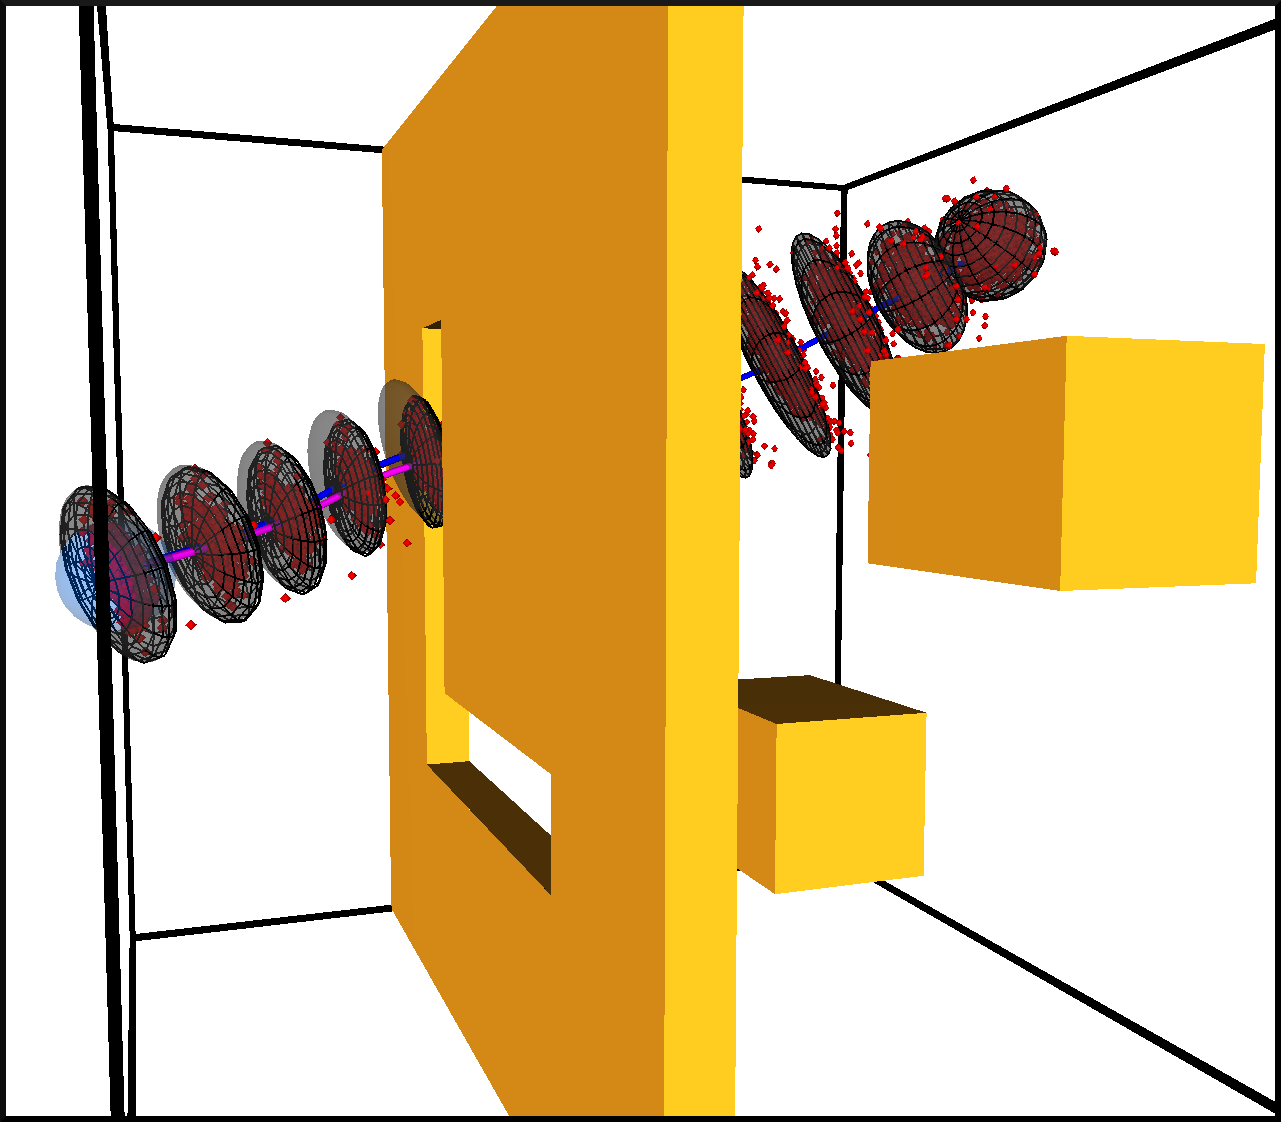
\includegraphics[width=160pt,clip]{figures/needle3d/plan1.png}}
\subfigure[\label{fig:2a}]{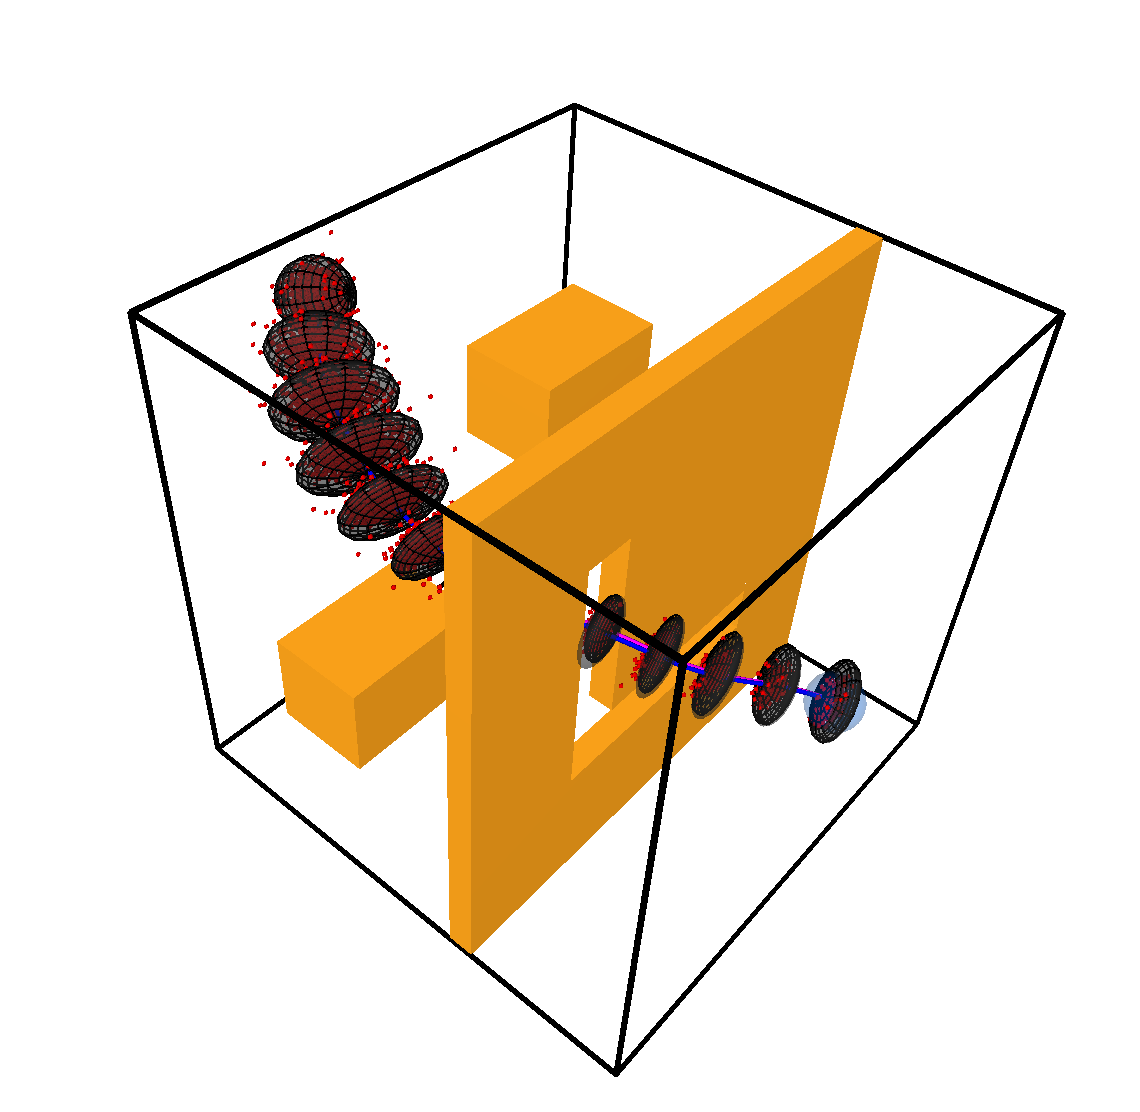
\includegraphics[trim=0pt 30pt 0pt 0pt, clip, width=160pt,clip]{figures/needle3d/plan1-top.png}}
\hfill
\subfigure[\label{fig:2b}]{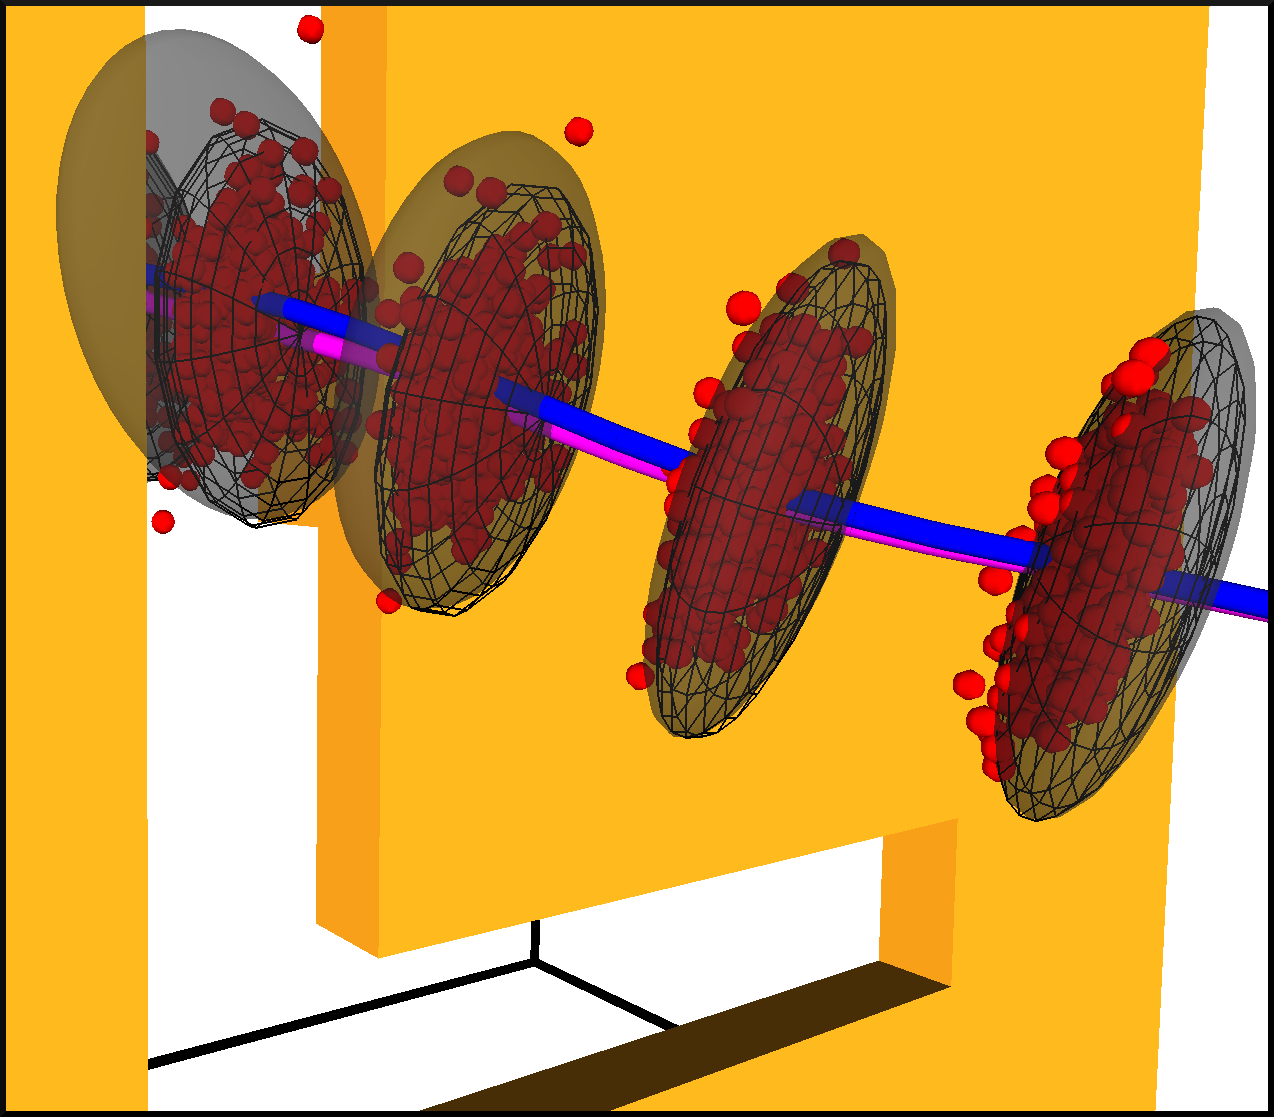
\includegraphics[width=160pt,clip]{figures/needle3d/plan1-closeup.png}}
\hfill
\subfigure[\label{fig:2c}]{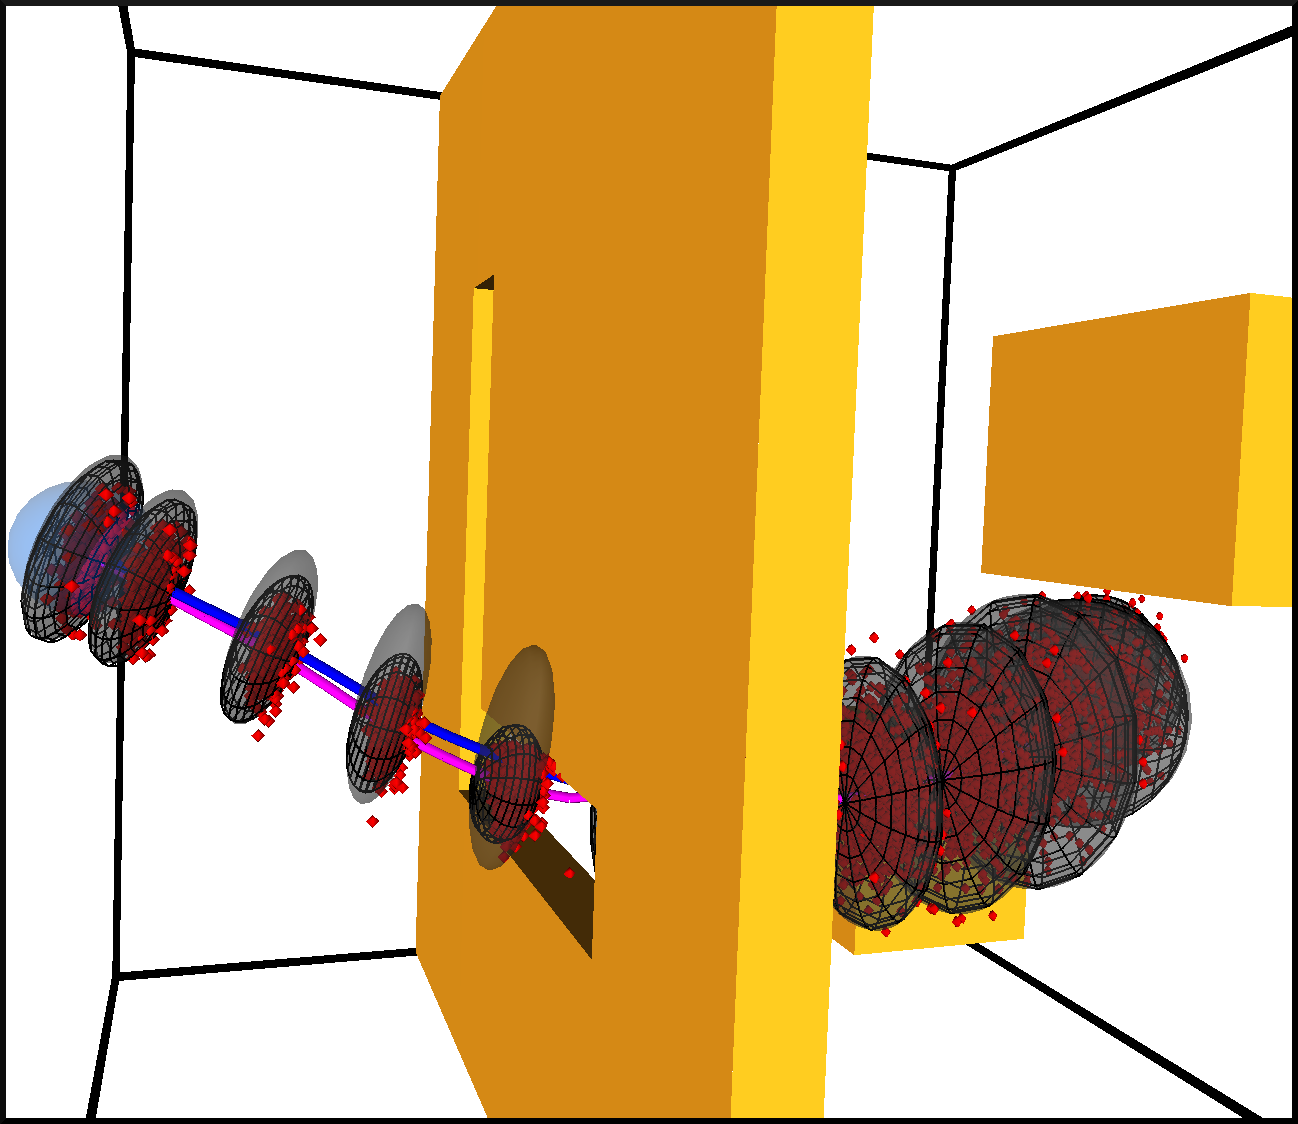
\includegraphics[width=160pt,clip]{figures/needle3d/plan2.png}}
{\,} \hfill
\vspace*{-5pt}
\caption{Nonholonomic bevel-tip steerable needle: (a) The unconditional distributions (solid gray ellipsoids, $3$ standard deviations) provide an overly conservative approximation of the uncertainty. Our method computes conditional distributions (black wireframe ellipsoids, $3$ standard deviations), which provide an accurate estimate of the probability distributions of the feasible robot states (shown in red). The probability of collision estimated by our method for the given plan is $54.5\%$, while the probability determined by Monte-Carlo simulations is $50.4\%$. Our method provides an accurate, yet conservative approximation of the collision probability. (b) Zoomed in view of the conditional distributions in the narrow corridor in the environment. The mean of the conditional distribution (magenta) deviates from the nominal plan due to the truncation. (c) The probability of collision estimated by our method for a second plan is $43.9\%$, while the probability determined by Monte-Carlo simulations is $42.2\%$.}
\vspace*{-15pt}
\label{fig:needle3d}
\end{figure*}

We also apply our method to a nonholonomic bevel-tip flexible needle \cite{Cowan2011_Chapter}, navigating in a 3D environment with obstacles. This class of needles offers improved mobility,
enabling needles to reach previously inaccessible targets while maneuvering around sensitive or impenetrable areas.

The state of the needle $\mathbf{x}$, is described by the $4 \times 4$ matrix $X = \left[\begin{smallmatrix} R & \mathbf{p} \\ \mathbf{0} & 1 \end{smallmatrix} \right] \in SE(3)$, where $\mathbf{p} \in \mathbb{R}^3$ is the position of the needle tip, and $R \in SO(3)$ is the rotation matrix that encodes the orientation of the needle tip, relative to a world coordinate frame. The needle naturally moves along constant curvature paths when inserted into tissue, but the curvature of the needle motion can be varied by duty cycled spinning of the needle during insertion. Under these modeling assumptions \cite{vandenBerg10_WAFR}, the control input $\mathbf{u} = [v, w, \kappa]^T \in \mathbb{R}^3$, consists of the insertion speed $v$, rotation speed applied at the base of the needle $w$, and the curvature $\kappa$.

It is convenient to describe the dynamics of the needle tip in terms of the instantaneous twist $U \in se(3)$ expressed in a local coordinate frame attached to the needle tip, given by:
\begin{equation}
U = \begin{bmatrix} [\mathbf{w}] & \mathbf{v} \\ \mathbf{0} & 0 \end{bmatrix}, ~ \mathbf{w} = \begin{bmatrix} v\kappa & 0 & w \end{bmatrix}^T, ~ \mathbf{v} = \begin{bmatrix} 0 & 0 & v \end{bmatrix}^T,
\end{equation}
where the notation $[\mathbf{s}]$ for a vector $\mathbf{s} \in \mathbb{R}^3$ refers to the $3 \times 3$ skew-symmetric cross-product matrix. The instantaneous twist $\tilde{U}$ that encodes the additive motion noise $\mathbf{m} = [\tilde{\mathbf{v}} ~ \tilde{\mathbf{w}}]^T \sim  \mathcal{N}[\mathbf{0}, M]$, can be similarly expressed.

Given a time step $\tau$, the stochastic discrete-time dynamics of the needle-tip is given by the following model:
\begin{equation}
\mathbf{f}[\mathbf{x}, \mathbf{u}, \mathbf{m}] = X\mathrm{exp}(\tau (U + \tilde{U})).
\end{equation}

We also assume that we receive partial, noisy feedback on only the position of the needle tip $\mathbf{p}$, and not its orientation. This is a reasonable assumption since current medical imaging
technologies such as ultrasound do not allow for measuring the full state of the needle tip (as the imaging resolution is often too low to infer its orientation). The noise in the
sensor measurement is modeled as $\mathbf{n} \sim \mathcal{N}[\mathbf{0}, N]$. This gives the following stochastic measurement model:
\begin{equation}
\mathbf{h}[\mathbf{x}, \mathbf{n}] = \mathbf{p} + \mathbf{n}.
\end{equation}
We follow the approach suggested in \cite{vandenBerg10_WAFR} to approximate the given nonlinear dynamics and measurement models with local linearizations around the nominal plan.

We consider a non-convex environment with a L-shaped narrow corridor and other obstacles to evaluate the performance of our method (Fig. \ref{fig:2a}). Fig. \ref{fig:2b} shows the discrepancy between the unconditional and conditional distributions in the presence of obstacles. The conditional distributions computed using our method provide an accurate estimate of the distribution of the collision free robot states along the plan, thus providing an accurate estimate of the probability of collision.

Similar to the analysis performed for the previous example, we generated a set of $100$ plans using the RRT planner starting from the goal state. We estimated the probability of collision using our method for each of these plans. This took $1.4$ seconds. We also used a brute-force approach to estimate the ground truth probability of collision using Monte-Carlo sampling. We performed $10,000$ simulations of executions of each plan with artificially generated motion and measurement noise, and counted the number of collision free executions. This took $388$ seconds, which is orders of magnitude slower than our method.

Table \ref{tab:comp} shows the results of how our method compares to the ground truth and prior approaches. For the given example, the mean error in estimation using our method as compared to the ground truth probability is $5.0\%$. The estimate computed using our method is much more accurate than the collision quality metric provided by LQG-MP (MAE $61.7\%$) \cite{vandenBerg11_IJRR} and the collision probability computed using the unconditional distributions directly by assuming independent probabilities (MAE $20.7\%$) \cite{Vitus11_ICRA}, while incurring negligible computational overhead. 

\section{Conclusion and Future Work} \label{sec:discussion}
We have presented an analytical method to estimate a priori the probability of collision for a mobile robot operating under Gaussian motion and sensing uncertainty. We have shown that it is necessary to consider the correlations between the a priori probability distributions of the robot state, to accurately estimate the true distributions and consequently, the probability of collision. We have also proposed a novel method for approximating the distribution of feasible states with truncated Gaussian distributions. Our method is directly applicable to a variety of motion planning under uncertainty methods \cite{vandenBerg11_IJRR, Vitus11_ICRA, Bry11_ICRA, vandenBerg11_ISRR, Toussaint09_ICML} to improve the quality and safety of the computed plans.

We plan to integrate our method with other motion planning under uncertainty methods, including improving the safety of computed plans in deformable environments \cite{Patil11_RSS}, and elegantly handle state constraints in optimization based approaches \cite{vandenBerg11_ISRR}. We also plan to extend our method to handle more general cases where the orientation of the robot is also relevant for collision detection. A natural extension is to investigate how our method can be extended to incorporate uncertainty in sensing obstacles in the environment \cite{Guibas08_WAFR}. Another interesting avenue for future research is to look at applications with unilateral contacts where the distribution of feasible states is no longer Gaussian \cite{Erez10_UAI}. It might be possible to approximate such non-Gaussian distributions using mixture of Gaussians and truncating them with respect to constraints on the robot state. 

\bibliographystyle{IEEEtranS}
\bibliography{ICRA2012-Patil}

\appendix[Truncated Gaussian Distributions]

Given a distribution $Y' \sim \mathcal{N}[\mu'_Y, \Sigma'_Y]$ and a joint Gaussian distribution $(X,Y)$:
\begin{equation} \label{eq:jointdist}
(X, Y) \sim \mathcal{N}\Bigg[\begin{bmatrix} \mu_X \\ \mu_Y \end{bmatrix}, \begin{bmatrix} \Sigma_X & \Sigma_{XY} \\ \Sigma_{YX} & \Sigma_Y \end{bmatrix}\Bigg],
\end{equation}
the conditional distribution $(X | Y = Y')$ is given by \cite{Book:Rasmussen06}:
\begin{equation} \label{eq:conditional}
(X | Y = Y') \sim \mathcal{N}[\mu_X - L(\mu_Y - \mu'_Y), \Sigma_X - L(\Sigma_Y - \Sigma'_Y)L^T]
\end{equation}
where $L = \Sigma_{XY}\Sigma^{-1}_Y$.

We can construct the joint distribution of the conditional distribution $\mathbf{y}_{t|t-1} \sim \mathcal{N}[\hat{\mathbf{y}}_{t|t-1}, R_{t|t-1}]$, and the transformed 1D distribution $y^i_{t|t-1} \sim \mathcal{N}[\tilde{\mathbf{a}}_i^T\hat{\mathbf{y}}_{t|t-1}, \tilde{\mathbf{a}}_i^T R_{t|t-1} \tilde{\mathbf{a}}_i]$, according to Eqn. (\ref{eq:jointdist}) as:
\begin{equation}
(\mathbf{y}_{t|t-1}, y^i_{t|t-1}) \sim \mathcal{N}\Bigg[\begin{bmatrix} \hat{\mathbf{y}}_{t|t-1} \\ \tilde{\mathbf{a}}_i^T\hat{\mathbf{y}}_{t|t-1} \end{bmatrix}, \begin{bmatrix} R_{t|t-1} & R_{t|t-1} \tilde{\mathbf{a}}_i \\ \tilde{\mathbf{a}}_i^T R_{t|t-1} & \tilde{\mathbf{a}}_i^T R_{t|t-1} \tilde{\mathbf{a}}_i \end{bmatrix}\Bigg].
\end{equation}

Using Eqn. (\ref{eq:conditional}), we reconstruct the truncated mean and variance of the joint distribution by conditioning on the truncated 1D distribution $y^i_{t|t} \sim \mathcal{N}[\mu_i, \sigma_i^2]$ (Eqn. \ref{eq:1DtruncMu}, \ref{eq:1DtruncSigma}), according to:
\begin{align}
&(\mathbf{y}_{t|t-1} | y^i_{t|t-1} = y^i_{t|t}) \sim \nonumber \\
&\mathcal{N}[\hat{\mathbf{y}}_{t|t-1} - L(\tilde{\mathbf{a}}_i^T\hat{\mathbf{y}}_{t|t-1} - \mu_i), R_{t|t-1} - L(\tilde{\mathbf{a}}_i^T R_{t|t-1} \tilde{\mathbf{a}}_i - \sigma_i^2)L^T],
\end{align}
where $L = \frac{R_{t|t-1} \tilde{\mathbf{a}}_i}{ \tilde{\mathbf{a}}_i^T R_{t|t-1} \tilde{\mathbf{a}}_i}$, which is exactly as in Eqns. (\ref{eq:truncmean}, \ref{eq:truncvar}). 

\end{document} 